\chapter{Teil 1 Mechanik}
\section{Einleitung}
\section{Aufgabenstellung und Zielsetzung}

Ziel ist es eine Katzenfütterungsanlage zu entwickeln. Ausgangslage sind Katzenfutterbeutel aus Aluminium-Kunststoff-Folie, die zeitlich gesteuert das Futter in den Behälter füllen sollen. Das Futter soll der Katze zugänglich gemacht werden und die leeren Beutel geruchsisoliert entsorgt werden. Die Anlage soll zum Beispiel während Kurzurlauben oder zum normalen Füttern der Katze oder des Hundes verwendet werden. Nach Aktivieren der Anlage wird in davor gewählten definierten Zeitpunkten die Katze gefüttert. 


\section{Problematik}

Jede Variante in den unten beschrieben Maschinen weisen Schwächen bzw. Probleme auf. Diese werden in den folgenden Punkten erläutert.

\subsection{Problematik des automatisierten Aufschneidens}

Das Problem des automatischen Schneiden ist, dass das Material der Verpackung sehr zäh ist und eine hohe Zugfestigkeit hat. Darum wird eine hoher Anpressdruck der Klingen erwartet. Zudem darf die Klinge, auch wenn sie lang ist, nicht verbiegen. Damit die Aluminium-Kunststoff-Folie nicht zwischen den Klinge gelangt und diese auseinander presst. Das hat Zufolge, dass das die Packung zerknittert und schwerer zu schneiden ist. 

\subsection{Problematik der Dichtheit bei Klemmen}

Bei der zweiten Variante wird erwartet das der Besitzer die Packung aufschneidet und eine Klemme befestigt. Diese muss mindestens fünf Tage lang dicht halten damit die Maschine nicht verschmutzt und die Katze etwas zu fressen hat. Wenn die Katzenfutterpackung nicht dicht ist gelangt Luft hinein und das gesamte Futter trocknet ein, somit lässt sich das ganze Futter noch schwerer aus der Verpackung pressen. Ein weiterer Nebeneffekt ist, das Schädlinge in die Packung gelangen können und die Katze, da sie wählerisch sein kann, das Futter nicht frisst.

\subsection{Problematik bei Entleerung der Verpackung}

Beim Entleeren der Verpackung bei geleeartiger Füllung treten einige Probleme auf die sich meist nur mit dem Pressen der Verpackung lösen lassen. Das Futter kann erstens in der Verpackung auf der Folie haften und somit durch die Schwerkraft nicht vollständig entleert werden. Zweitens die Luft muss von der Öffnung bis zur geschlossenen Seite gelange, damit der Luftdruck nicht das Entleeren verhindert(ähnlich wie beim Entleeren einer volle Ketchupflasche). 

\subsection{Problematik vom Geruch}

Bei automatischen Füttern eine Katze ist der Geruch ein großes Problem, da Katzenfutter schon am ersten Tag einen strengen Geruch hat und der sich über die Tage steigert. Die einzige Maßnahme die getroffen werden kann, ist die ganze Maschine Luftdicht zu gestalten (die einzige Ausnahme wäre, wenn es dem Benutzer nicht stört und dieser erleichtert ist wenn seine Katze gefüttert ist). 

\subsection{Problematik von der Reinigung nach dem Urlaub}

Durch das Pressen der Packungen kann das Gelee an der Walze bleiben und diese verschmutzen. Die gedachte Lösung ist, dass das Gehäuse aufklappbar ist. Das bedeutet dass der Benutzer mit viel Freiraum in die Maschine greifen kann und  somit die beiden Walzen reinigen. Die Futterschüsseln lassen sich durch die Konstruktion der unten beschriebene Variante (Drehplatte) leicht entfernen lassen. Die Futterplatte kann bei eines Falles einer Verschmutzung durch ihre wasserfeste Beschichtung gereinigt werden.

\subsection{Problematik bei einfrieren des Futters}



\section{Konzepte} 

In den folgenden Punkten werden die verschiedenen Varianten vorgestellt. Weiters werden durch Schemenskizzen die einzelnen Varianten verdeutlicht um so einen Eindruck der zu realisierten Maschine zu erhalten.

\subsection{Variante 1: Automatisiertes Aufschneiden} 
\subsubsection{Übersicht der Prozessschritte}
\begin{itemize}
\item[1] Füllen des Futtermagazins
\item[2] Führen zur Schneidplatte
\item[3] Schnitt
\item[4] Pressen
\item[5] Entsorgen
\item[6] Füttern
\end{itemize}

\subsubsection{Füllen des Futtermagazins}

Im den folgenden Bildern wird mithilfe einer Lego-Darstellung gezeigt, wie das Magazin aus verschiedenen Blickwinkeln befüllt aussieht. Hier muss man beachten das die vom Hersteller zu öffneten Seite in Richtung des Schneidewerks zeigt (die schmale Seite mit der Einkerbung). Das ganze Förderband besteht grundsätzlich aus der Halterung die das Magazin in einer bestimmten Höhe hält, damit die einzelnen Trennwände nicht mit dem Boden kollidieren und somit keine freie Bewegung ermöglicht ist. Der Oberteil des Bandes schließt eben mit der Schneideplattenhöhe ab um ein leichtes gleiten der Packung durch den Greifer zu ermöglichen, ohne das es Höhenunterschiede überwinden muss. Weiters wird über zwei Räder ein Band gespannt an denen die Wände in Abstand der Dicke der Packung festgemacht werden. Das Band wird mithilfe eines Motors in Bewegung gebracht und kann somit von Abteil zu Abteil bewegt werden um immer nach dem füttern eine neue Packung bereit zu stellen. Auf diesem Band können je nach Länge eine gewissen Anzahl an Futterpackung gelegt werden, natürlich nur auf der Oberseite da die Packungen ansonsten aus den Abteilung fallen, weil sie nicht nach oben geschlossen sind.  Siehe Abbildungen: \ref{Magazin Vorne}, \ref{Magazin Seitlich}, \ref{Magazin Oben}

\begin{figure}[H]
\begin{center}
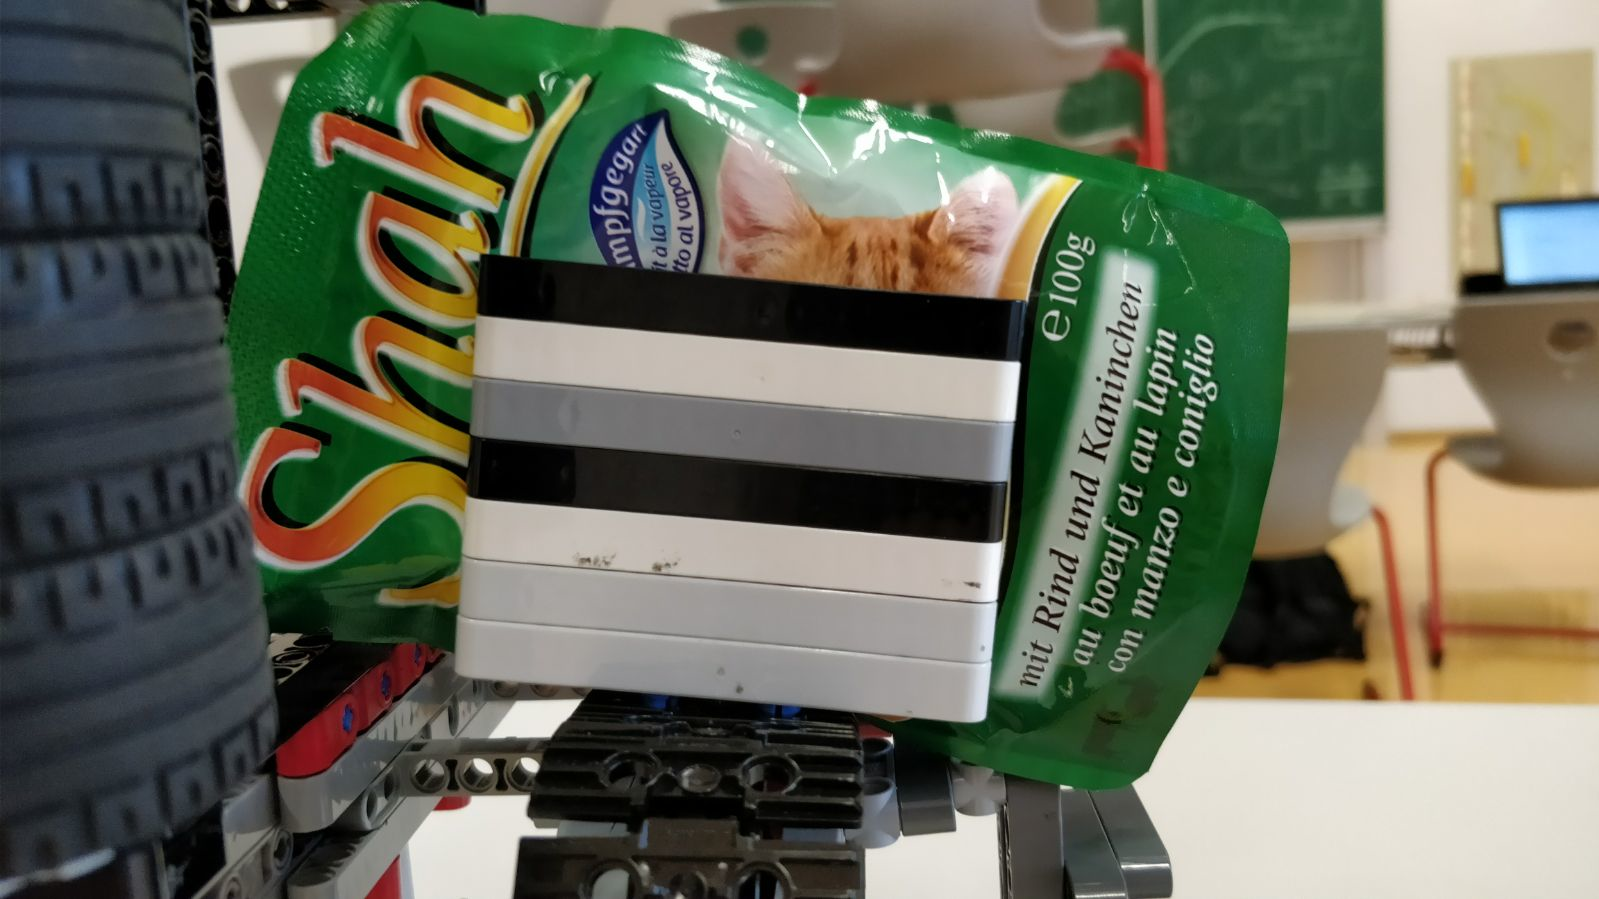
\includegraphics[width=13cm]{Bilder/Ablauf_1_png/Magazin_Vorne.png}
\caption{Magazin Vorne}
\label{Magazin Vorne}
\end{center}
\end{figure}

\begin{figure}[H]
\begin{center}
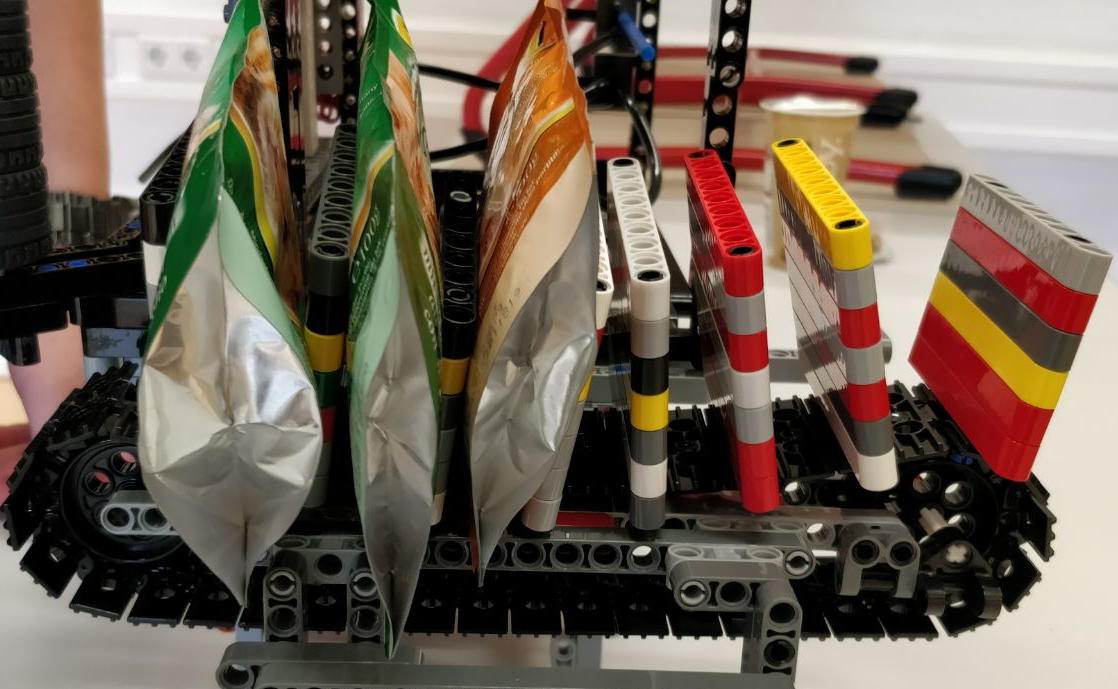
\includegraphics[width=13cm]{Bilder/Ablauf_1_png/Magazin_Seitlich.png}
\caption{Magazin Seitlich}
\label{Magazin Seitlich}
\end{center}
\end{figure}

\begin{figure}[H]
\begin{center}
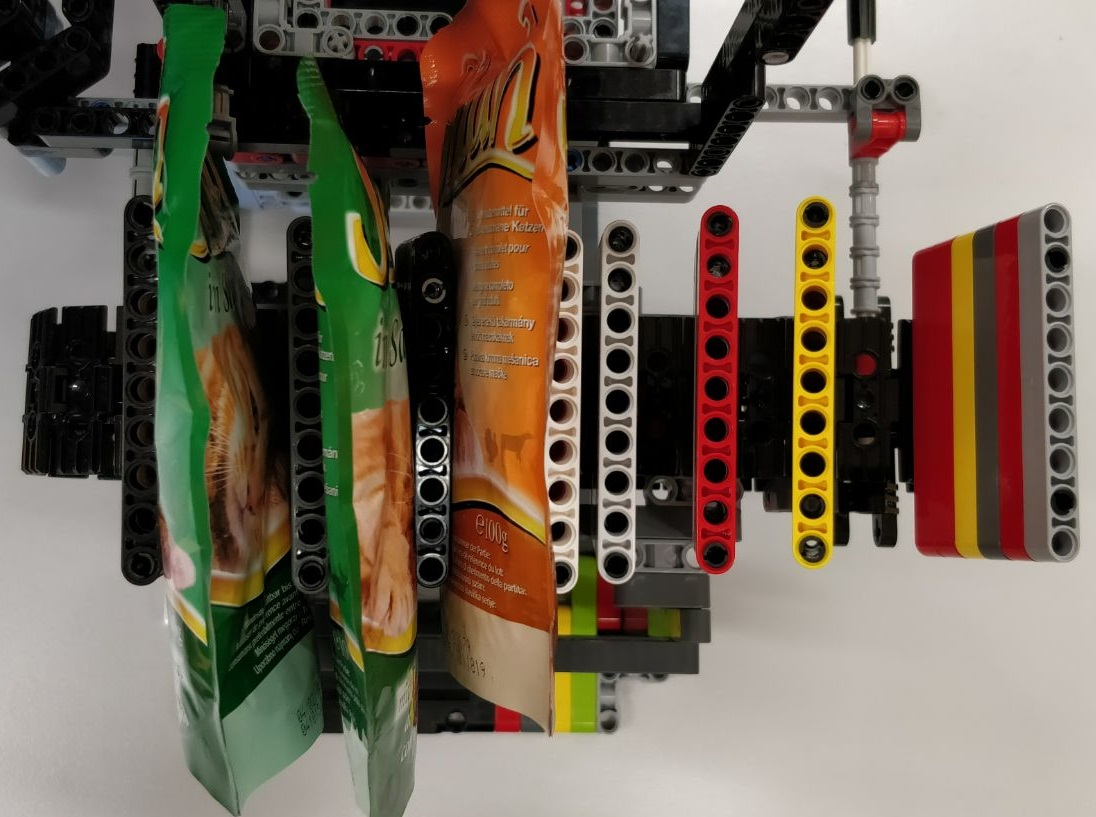
\includegraphics[width=13cm]{Bilder/Ablauf_1_png/Magazin_Oben.jpeg}
\caption{Magazin Oben}
\label{Magazin Oben}
\end{center}
\end{figure}

\subsubsection{Führen zur Schneidplatte}

In diesem Schritt wird mithilfe eines Greifers (dargestellt durch eine Hand) die Packung in richtiger Position gebracht.
Durch die richtige Höhe des Förderbandes muss der Greifer keine hohe Kraft besitzen um die Packung an ihrem Zielort zu bringen. Der Greifer dient auch noch dazu während des Schneidens neben den Magnetzylindern die Packung stabil an Stelle zu halten ohne dass der Schnittpunkt verrutscht und die Schneide nicht mehr die Einkerbung, die leichter zu Schneiden ist, trifft. Das kann zu dem Problem führen, dass man die dickere Kunstoffumhüllung schneidet und der Schnitt nicht Ordnungsgemäß durchgeführt wird. Dadurch kann der Kunstoff zwischen die Schneiden gelangen und sie damit auseinander drücken. Dadurch kann die Packung nicht aufgeschnitten werden. Siehe Abbildungen: \ref{Magazin Auszug}, \ref{Magazin Mitte}

\begin{figure}[H]
\begin{center}
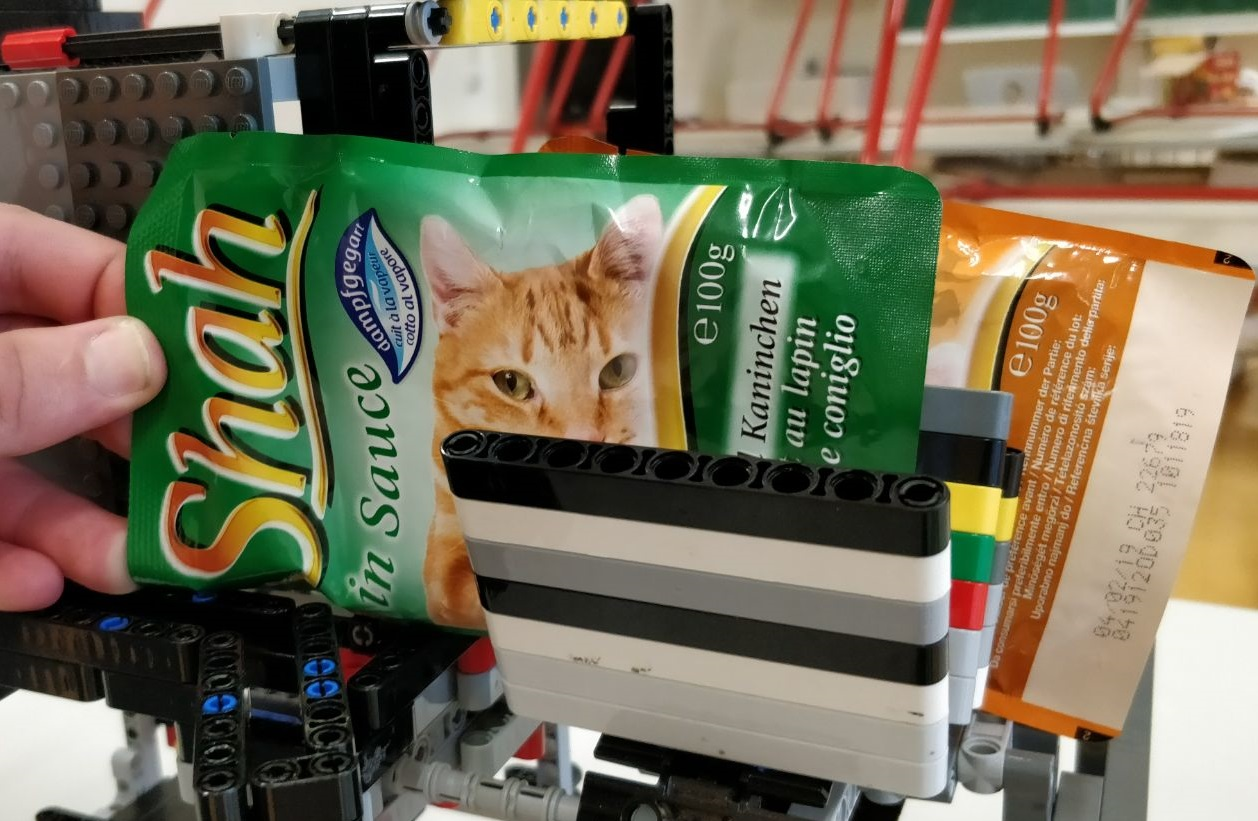
\includegraphics[width=13cm]{Bilder/Ablauf_1_png/Magazin_Auszug.jpeg}
\caption{Magazin Auszug}
\label{Magazin Auszug}
\end{center}
\end{figure}

\begin{figure}[H]
\begin{center}
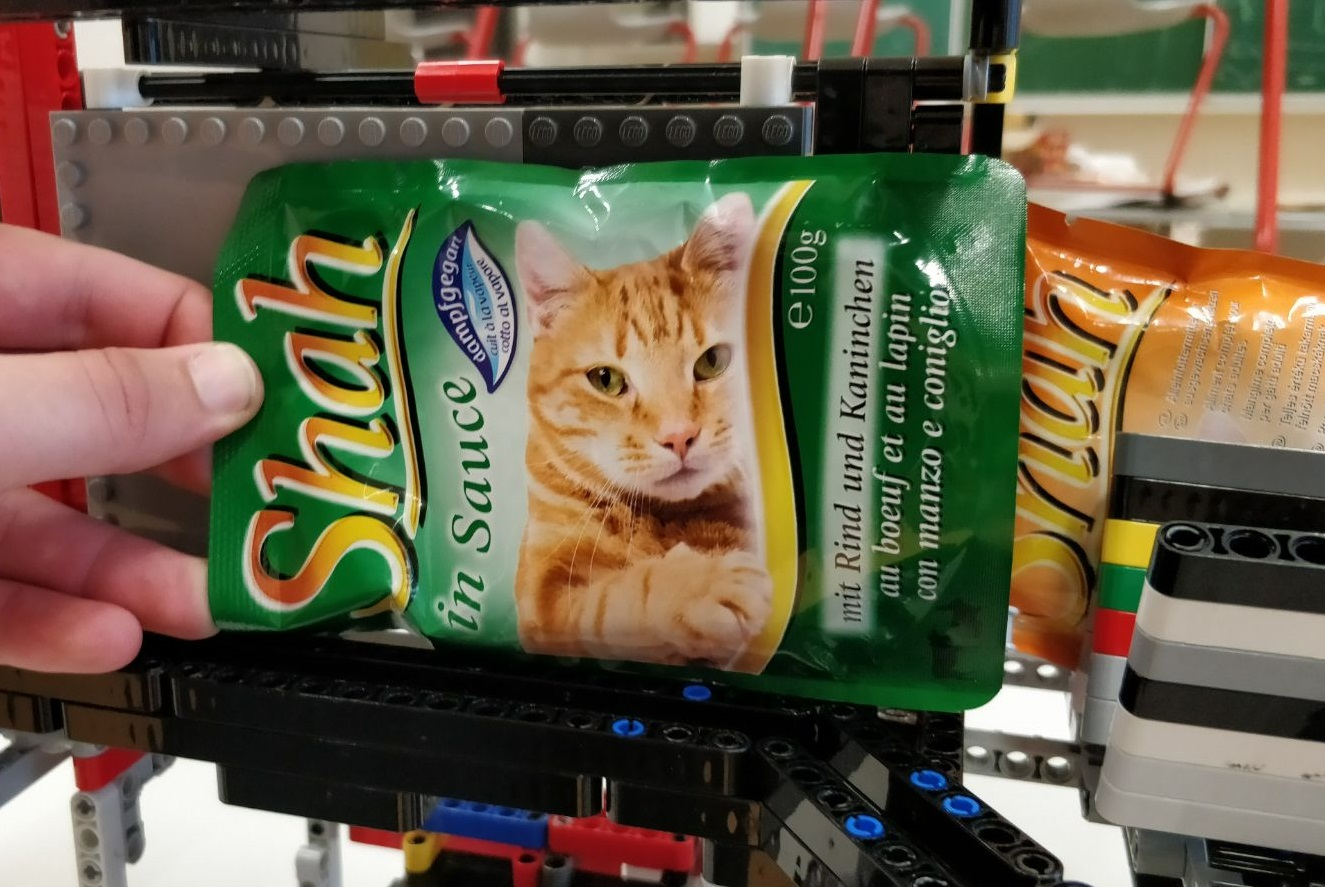
\includegraphics[width=13cm]{Bilder/Ablauf_1_png/Magazin_Auszug_2.jpeg}
\caption{Magazin Auszug Mitte}
\label{Magazin Mitte}
\end{center}
\end{figure}

Wie im Bild gezeigt liegt das Katzenfutterpackerl in der richtigen Position und wird mit zwei Magnetzylindern an der Schneidefläche festgehalten. Die Magnetzylinder haben genügend Kraft um die Packung auch während dem Schnitt und der Walzphase in Position zu halten. Wenn die Packung verrutschen würde könnte im schlimmsten Fall die Funktion der Maschine beeinflusst werden, indem sie den Greifer oder das Förderband blockiert. Daraufhin muss die Maschine manuell geöffnet und den Beutel per Hand raus geholt werden. Siehe Abbildung: \ref{Schneidebereit}

\begin{figure}[H]
\begin{center}
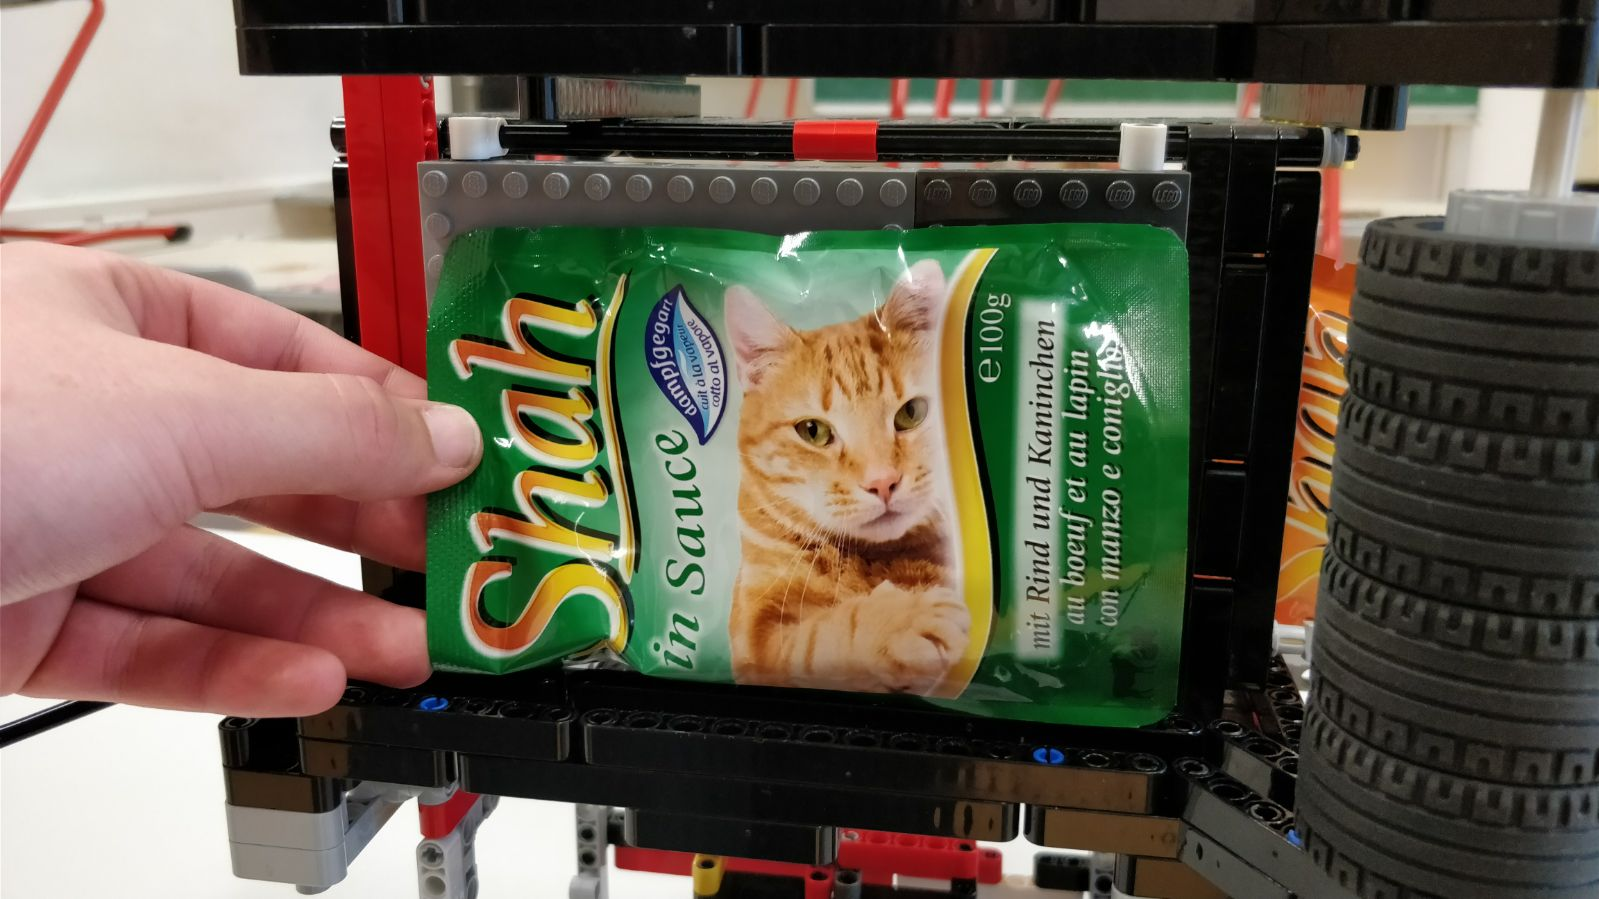
\includegraphics[width=13cm]{Bilder/Ablauf_1_png/Schneidebereit.jpeg}
\caption{Schneidebereit}
\label{Schneidebereit}
\end{center}
\end{figure}

\subsubsection{Schnitt}

In der richtigen Position muss man mit 2 scharfen Klingen mit viel Druck die Packung aufschneiden. Eine davon wird an der Schnittfläche angebracht und die andere macht die Schneidbewegung, wobei die beiden aneinander reibenden Kanten in einem Schnitt resultieren. Die Packung kann mit einem Schnitt vollständig geöffnet werden. Mit zu wenig Druck gelangt zu viel Kunstoffmaterial zwischen die Schneideflächen und durch die Länge der Schneiden biegen sie sich auseinander und somit kommt kein ordentlicher Schnitt zusammen. Bei öfteren Auftritts dieses besprochenen Problems bei der selben Packung kann es zufolge haben, dass sich die Packung nicht mehr mit der Maschine schneiden lässt, weil es sich durch die vielen Versuche verformt.  Siehe Abbildung: \ref{Schnitt}

\begin{figure}[H]
\begin{center}
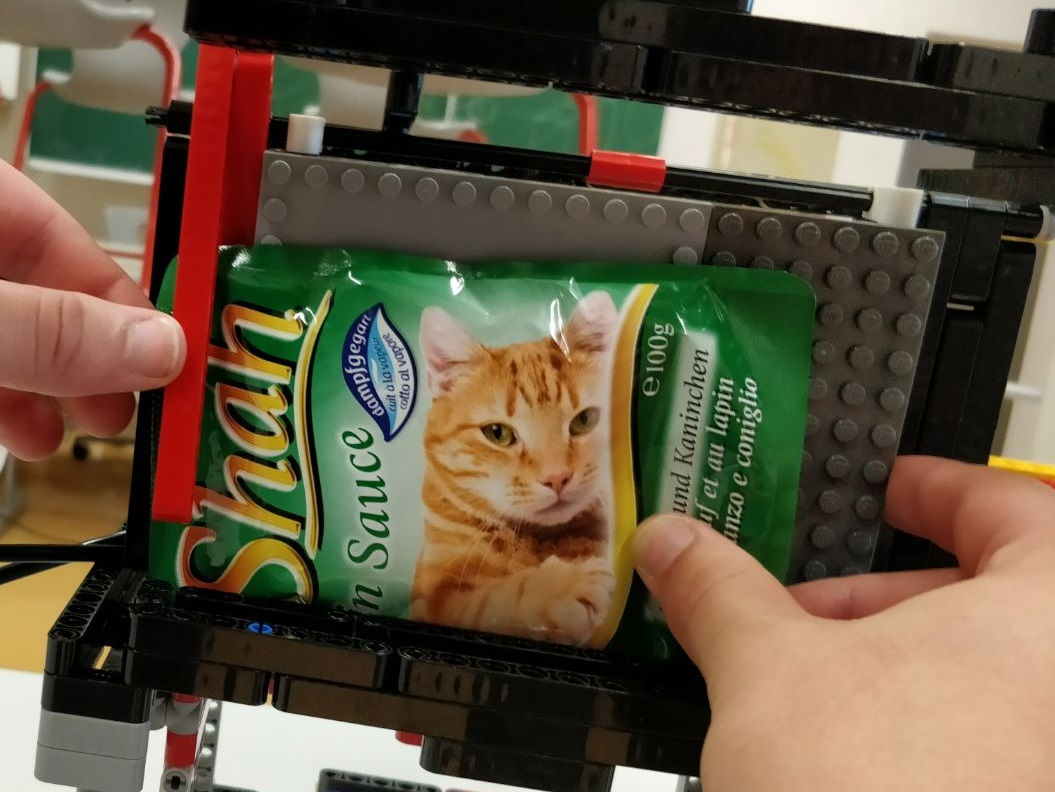
\includegraphics[width=13cm]{Bilder/Ablauf_1_png/Schnitt}
\caption{Schnitt}
\label{Schnitt}
\end{center}
\end{figure} 

\subsubsection{Pressen}

Nach dem Aufschneiden wird mit einer Rolle die Packung ausgepresst. Dazu werden zuerst die ersten 2 Magnetzylinder gelöst bis die Rolle vorbei ist. Danach werden sie wieder in Position gebracht. Daraufhin werden die anderen beiden gelöst und die Rolle fährt ans Ende. Die Rolle ist auf einer Welle platziert, diese wird mit 2 Sicherungsringen an einer  vorgegebenen Position befestigt. Die Rolle ist 10 cm breit, damit ohne Probleme die 9,4cm breite Futterpackung ausgepresst werden kann. Sie wird in einer Vorrichtung an der Maschine angehängt und steht mit einem bestimmten Winkel auf die Schneidfläche damit ein großer Anpressdruck entsteht. Durch die schmierige Konsistenz gleitet das Futter aus der Verpackung und wird nicht von der Walze zerquetscht. Nach der Beseitigung der Verpackung werden zuerst die beiden Magnetzylinder von der Maschine entfernt in Anfangsposition gebracht, damit die Walze ohne 6 in Startposition zurückkehren kann. Siehe Abbildungen: \ref{Ausquetschen Beginn}, \ref{Ausquetschen Mitte}, \ref{Ausquetschen Ende}

\begin{figure}[H]
\begin{center}
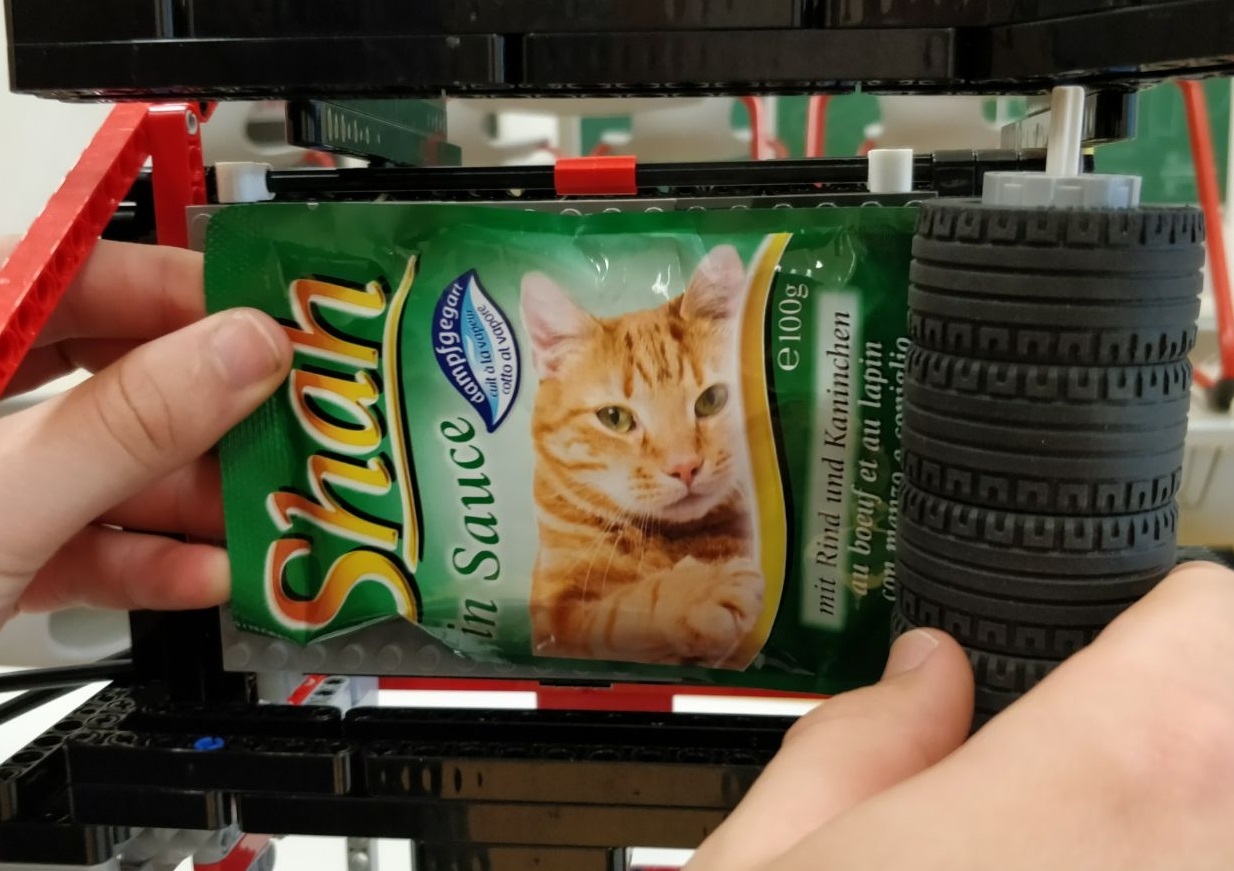
\includegraphics[width=13cm]{Bilder/Ablauf_1_png/Ausquetschen_1}
\caption{Ausquetschen Beginn}
\label{Ausquetschen Beginn}
\end{center}
\end{figure}

\begin{figure}[H]
\begin{center}
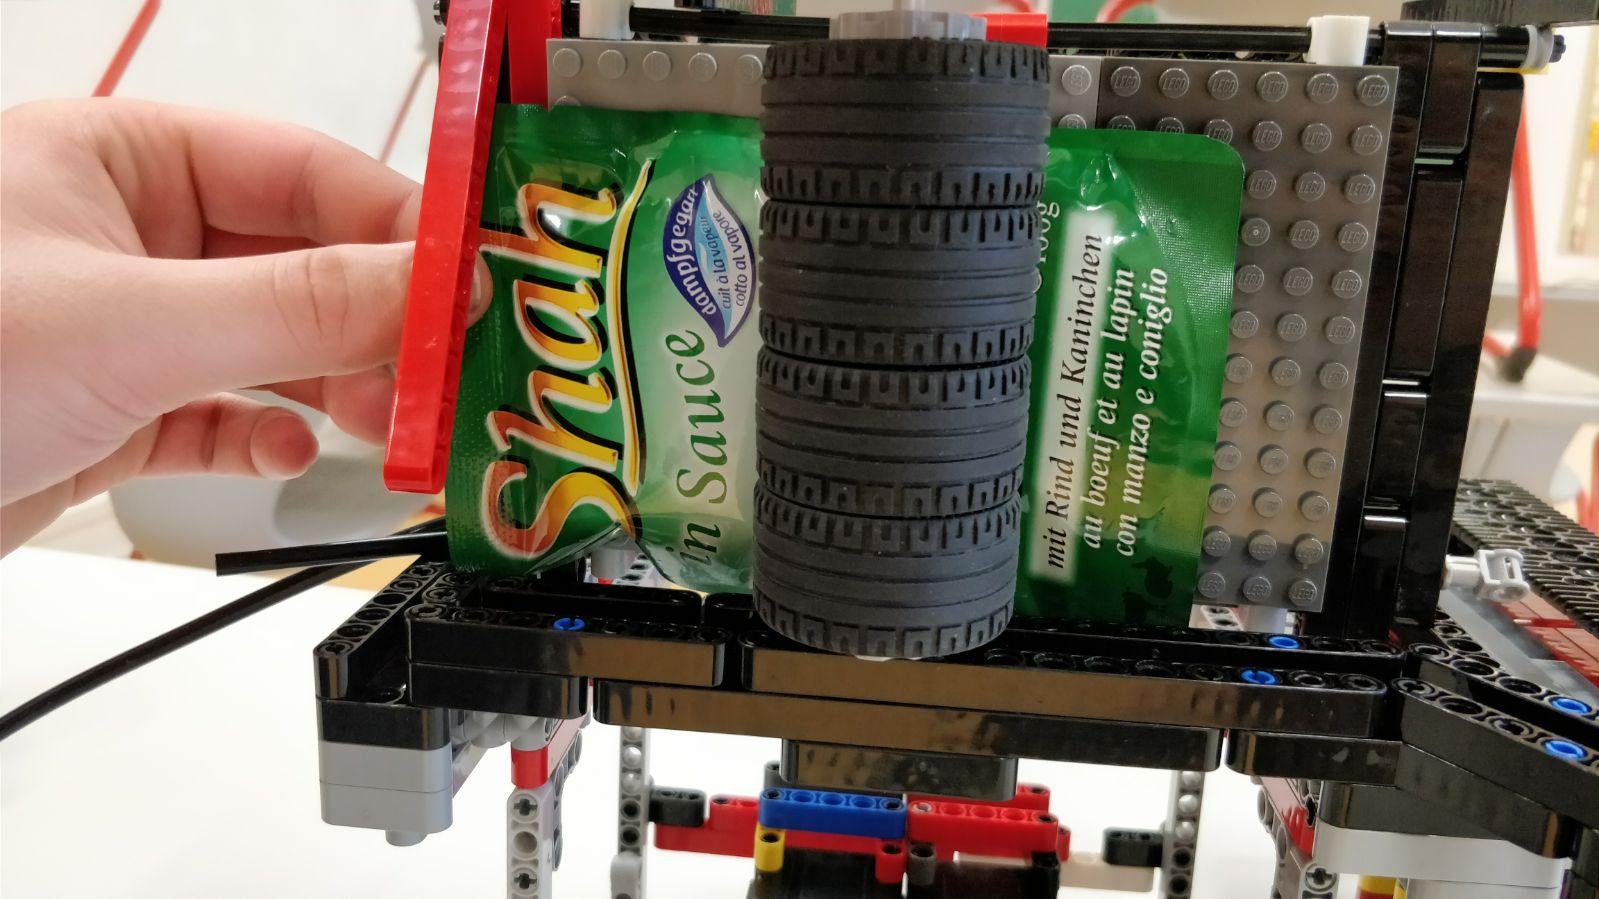
\includegraphics[width=13cm]{Bilder/Ablauf_1_png/Ausquetschen_2}
\caption{Ausquetschen Mitte}
\label{Ausquetschen Mitte}
\end{center}
\end{figure}

\begin{figure}[H]
\begin{center}
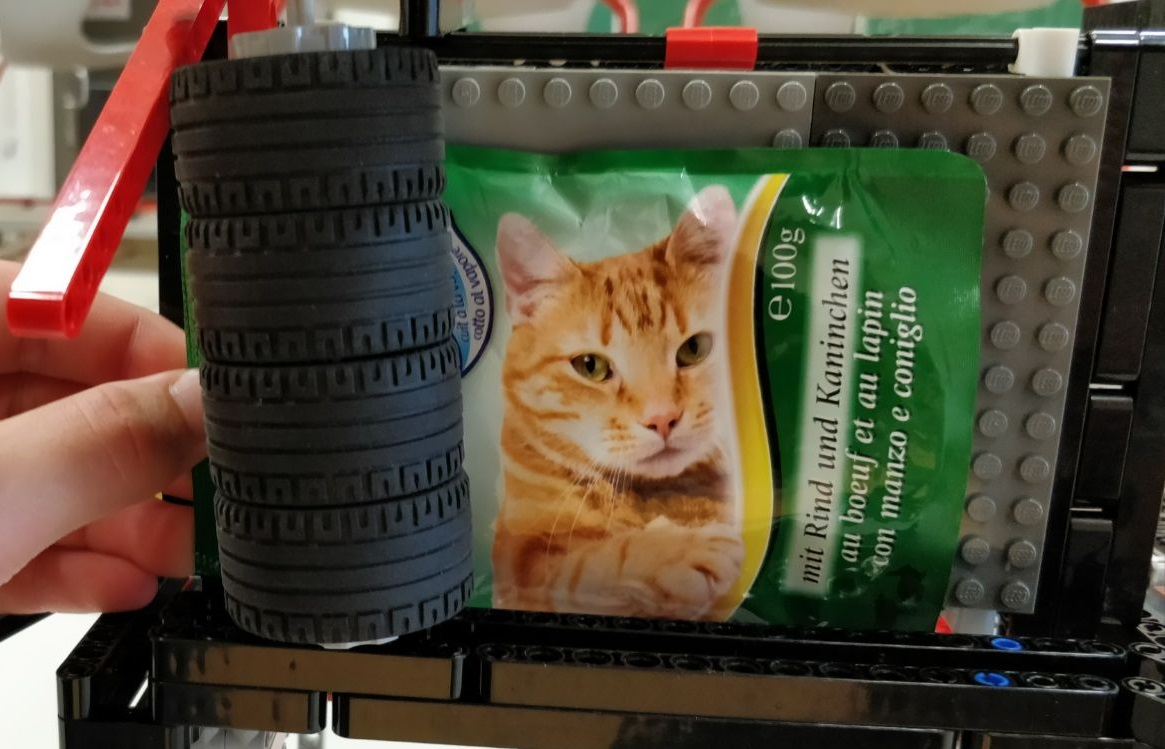
\includegraphics[width=13cm]{Bilder/Ablauf_1_png/Ausquetschen_3}
\caption{Ausquetschen Ende}
\label{Ausquetschen Ende}
\end{center}
\end{figure}
\newpage
\subsubsection{Entsorgen}

Nach dem Auspressen wird die leere Packung durch die Rückklappe in einen Luftdichten Container geworfen. Die Klappe wird durch zwei Stifte gehalten und lässt sich durch ein Scharnier nach hinten klappen. Die zwei Stifte sind mit Kosten verbunden da 2 Magnetzylinder benötigt werden und die in einem Schaltplan zu berücksichtigt sind. Außerdem benötigen sie zusätzlich Platz. Siehe Abbildung: \ref{Auswurf Beginn}, \ref{Fertiger Auswurf}

\begin{figure}[H]
\begin{center}
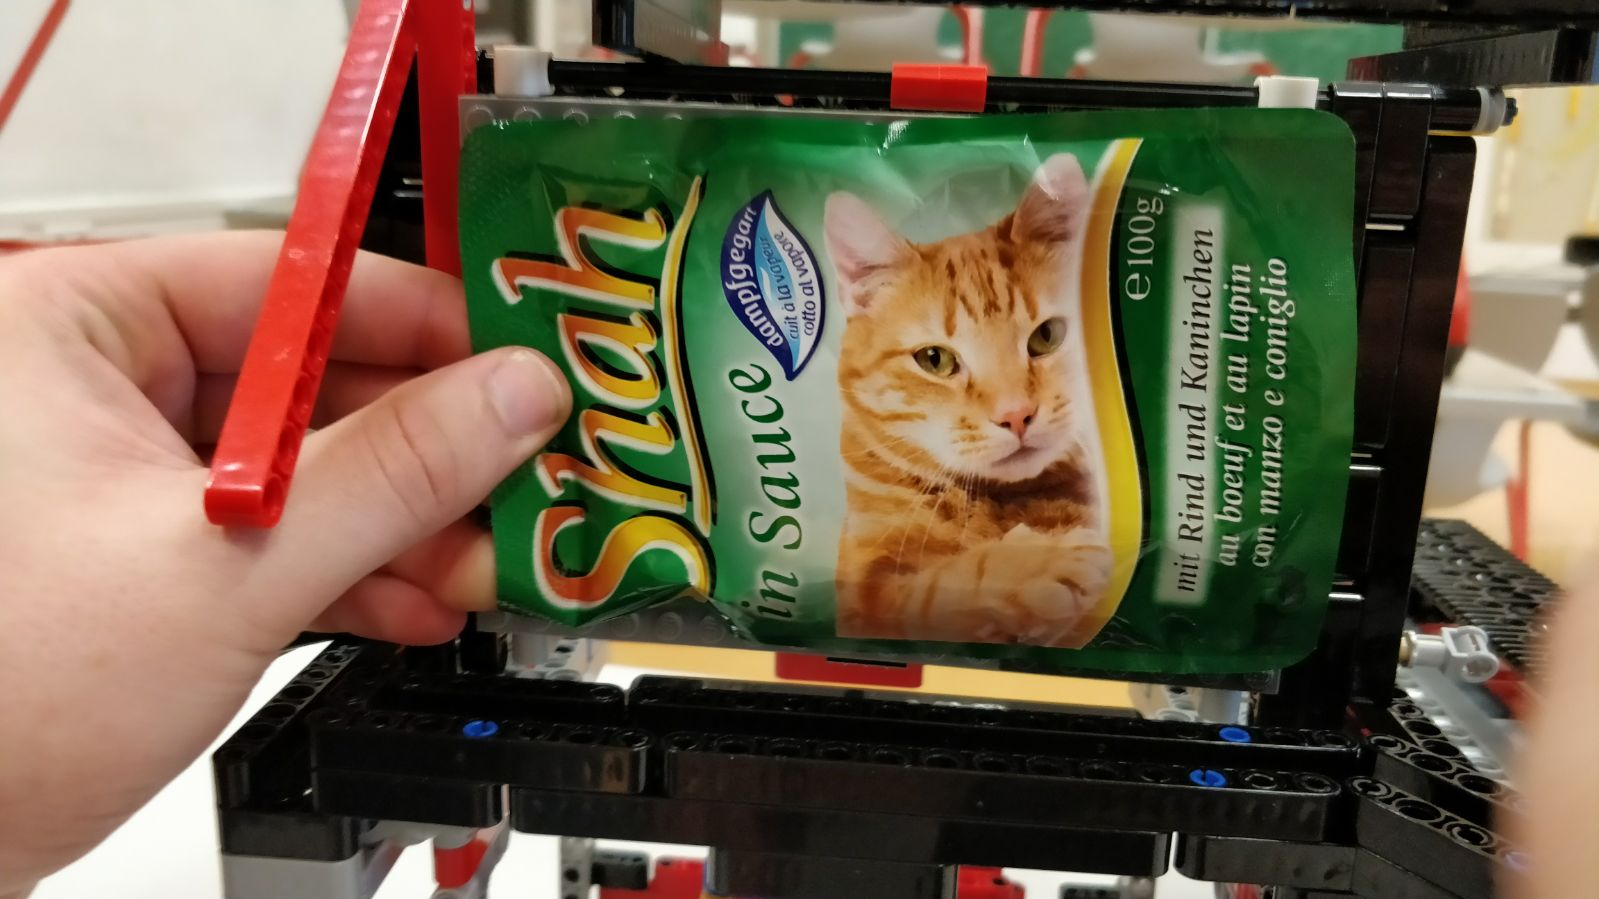
\includegraphics[width=13cm]{Bilder/Ablauf_1_png/Auswurf_1}
\caption{Auswurf Beginn}
\label{Auswurf Beginn}
\end{center}
\end{figure}

In der Abbildung: \ref{Bolzen drinnen} sieht man den Stift der ein vorzeitiges nach Hinten klappen verhindert. Die Stifte müssen so dimensioniert sein damit sie die Kräfte der Walze aushält.

\begin{figure}[H]
\begin{center}
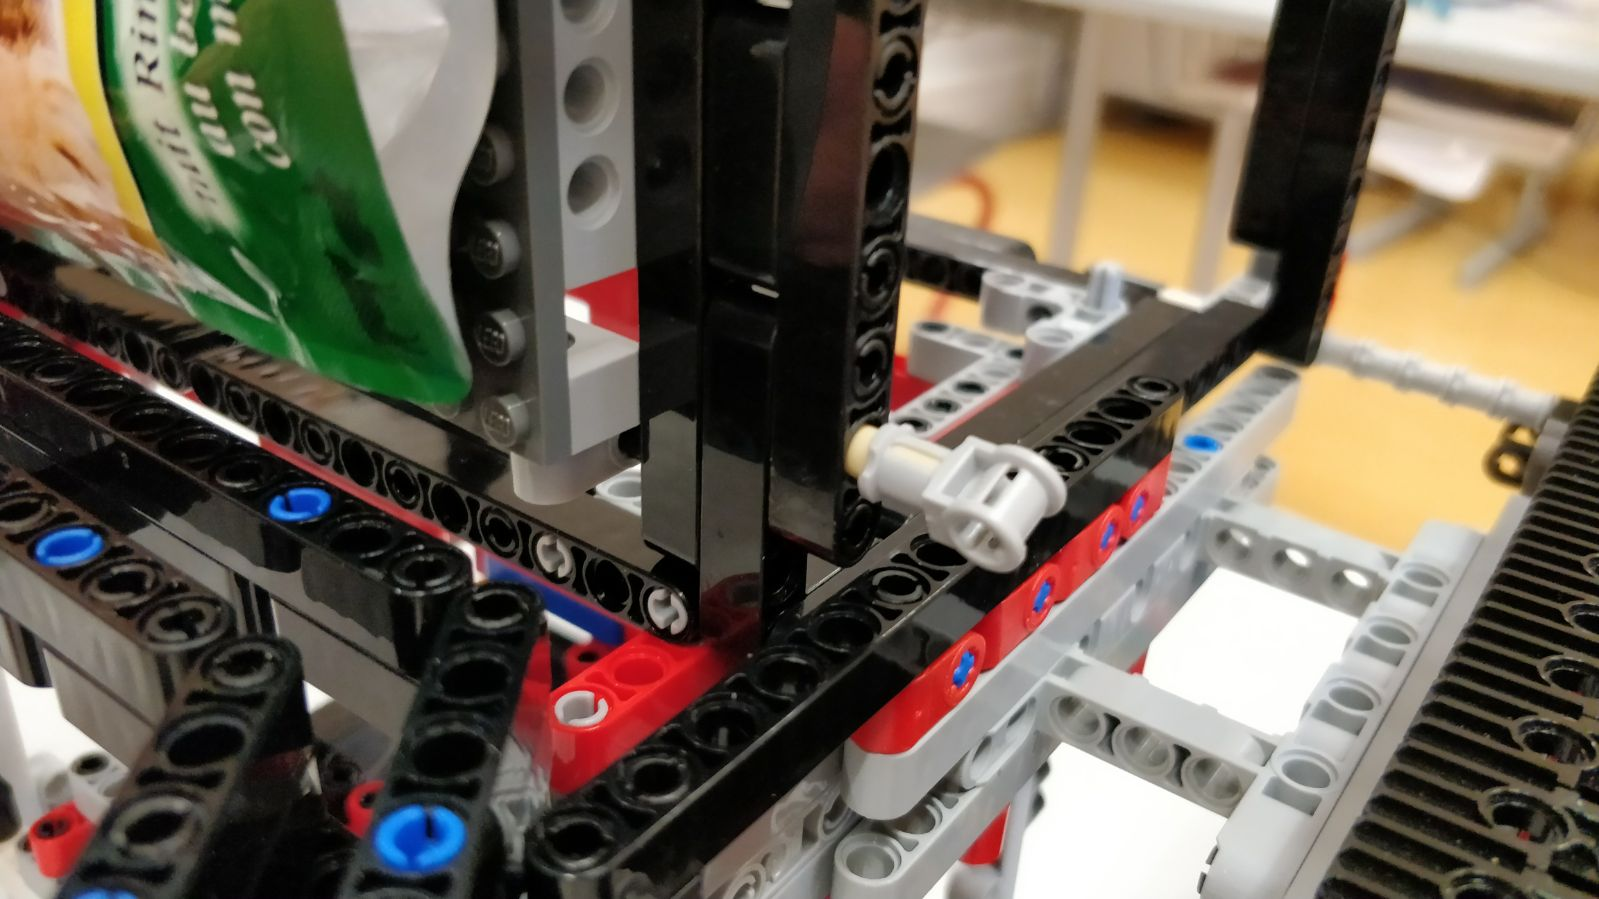
\includegraphics[width=13cm]{Bilder/Ablauf_1_png/Auswurf_2}
\caption{Bolzen drinnen}
\label{Bolzen drinnen}
\end{center}
\end{figure}


In der Abbildung: \ref{Bolzen entfernen} wurde der Bolzen entfernt und somit lässt sich die Klappe nach hinten klappen.

\begin{figure}[H]
\begin{center}
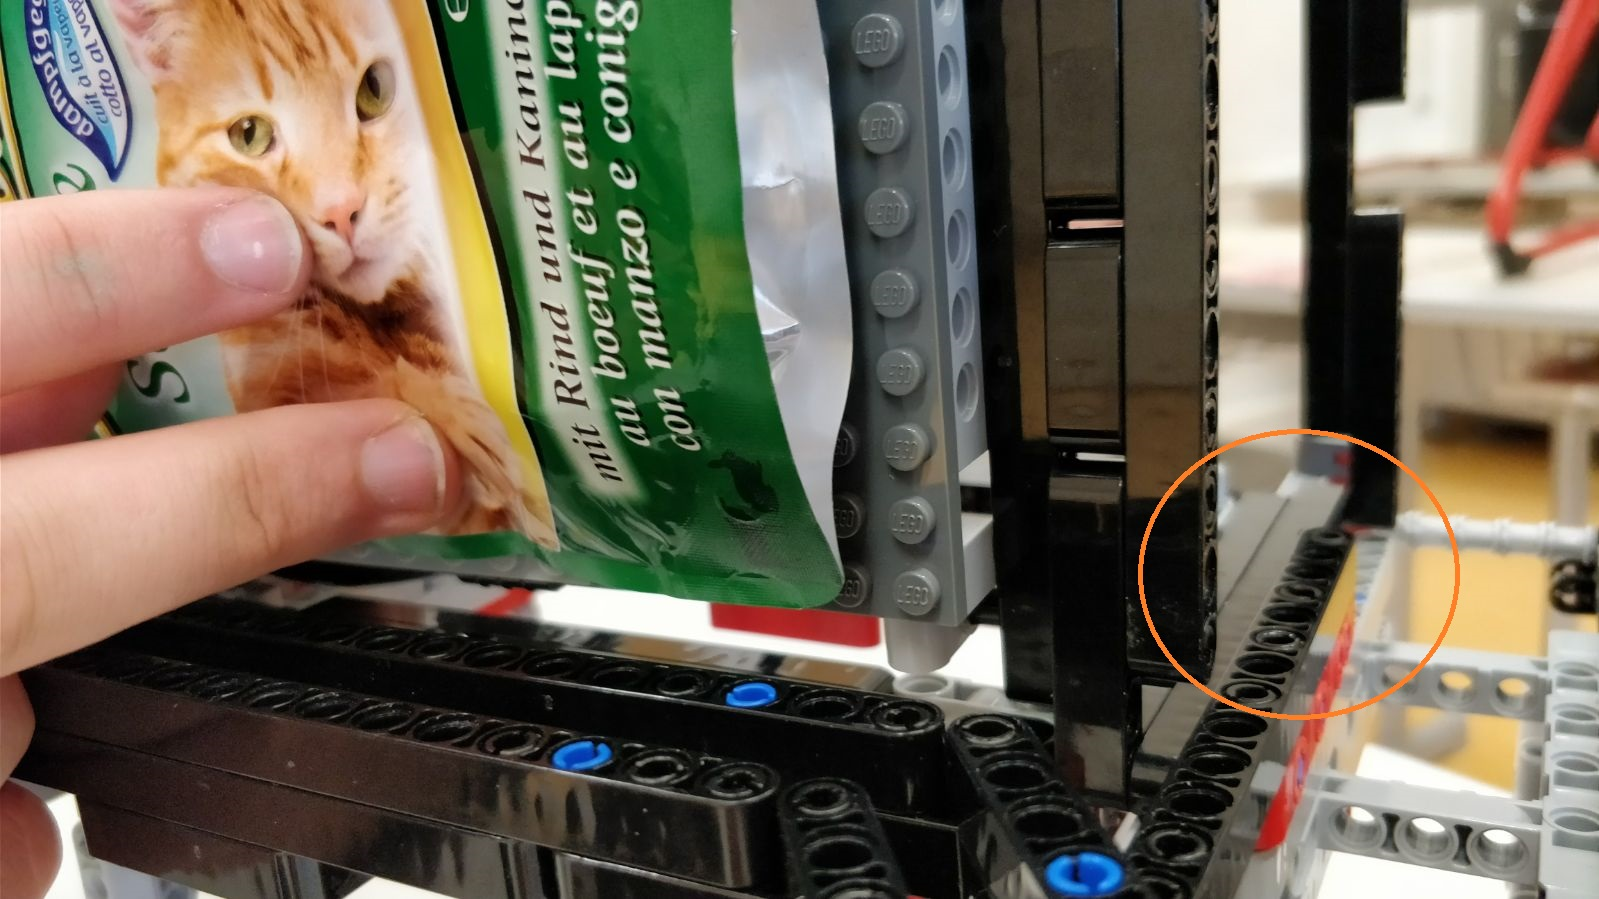
\includegraphics[width=13cm]{Bilder/Ablauf_1_png/Auswurf_3}
\caption{Bolzen entfernen}
\label{Bolzen entfernen}
\end{center}
\end{figure}

In der Abbildung: \ref{Klappe öffnen} wird demonstriert wie die Magnetzylinder die leere Packung gegen die Klappe drücken, wodurch die Klappe sich öffnet.

\begin{figure}[H]
\begin{center}
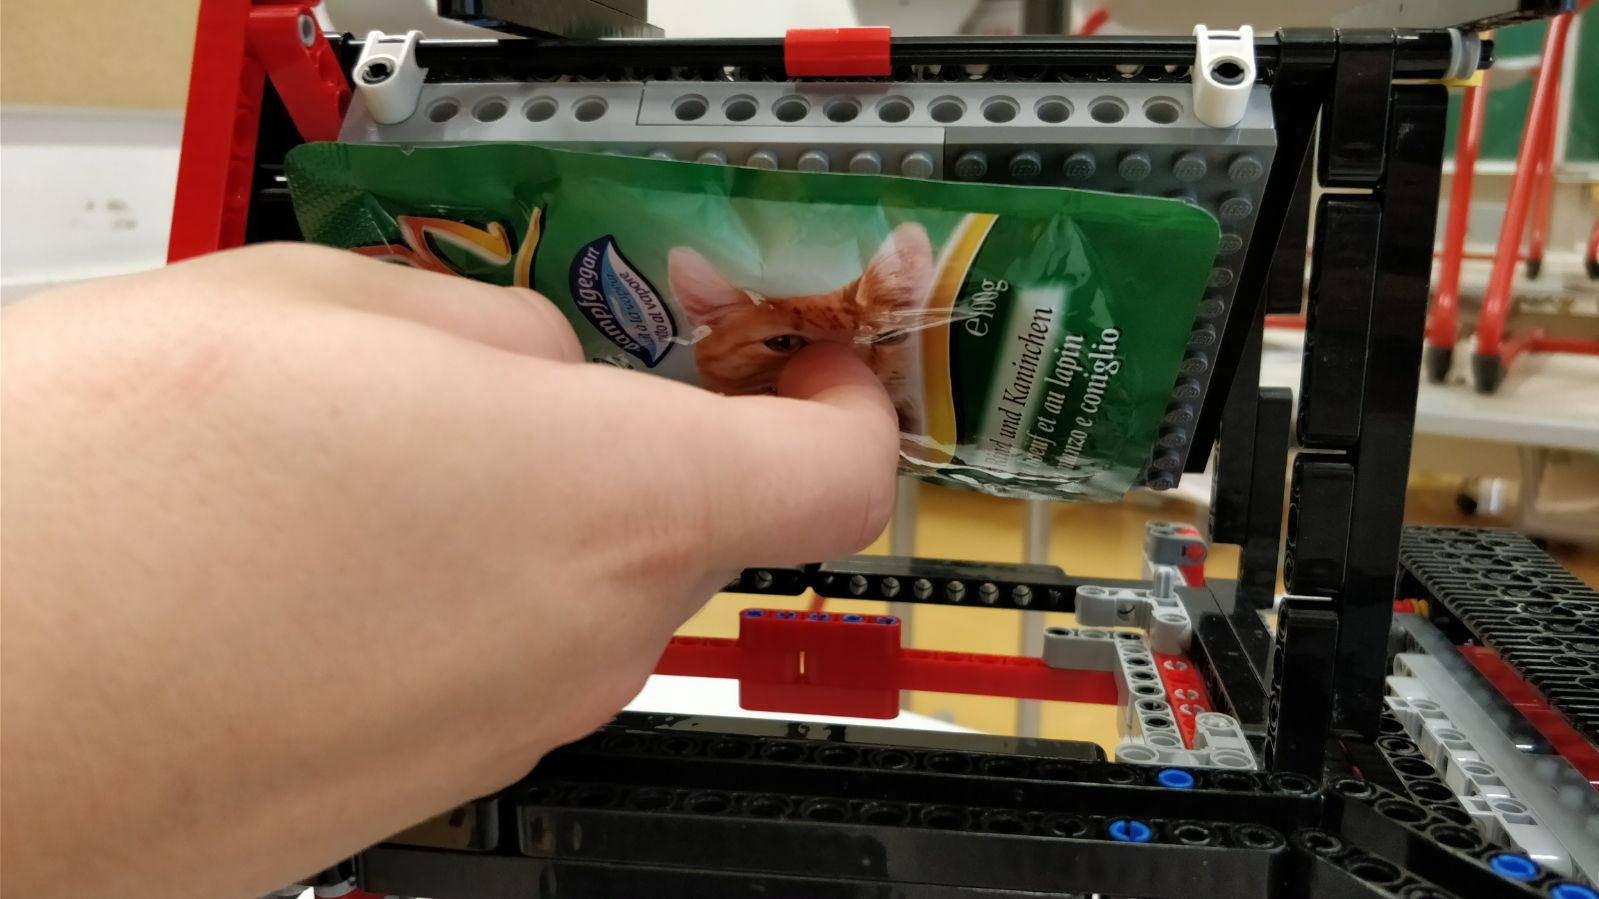
\includegraphics[width=13cm]{Bilder/Ablauf_1_png/Auswurf_4}
\caption{Klappe öffnen}
\label{Klappe öffnen}
\end{center}
\end{figure}

\begin{figure}[H]
\begin{center}
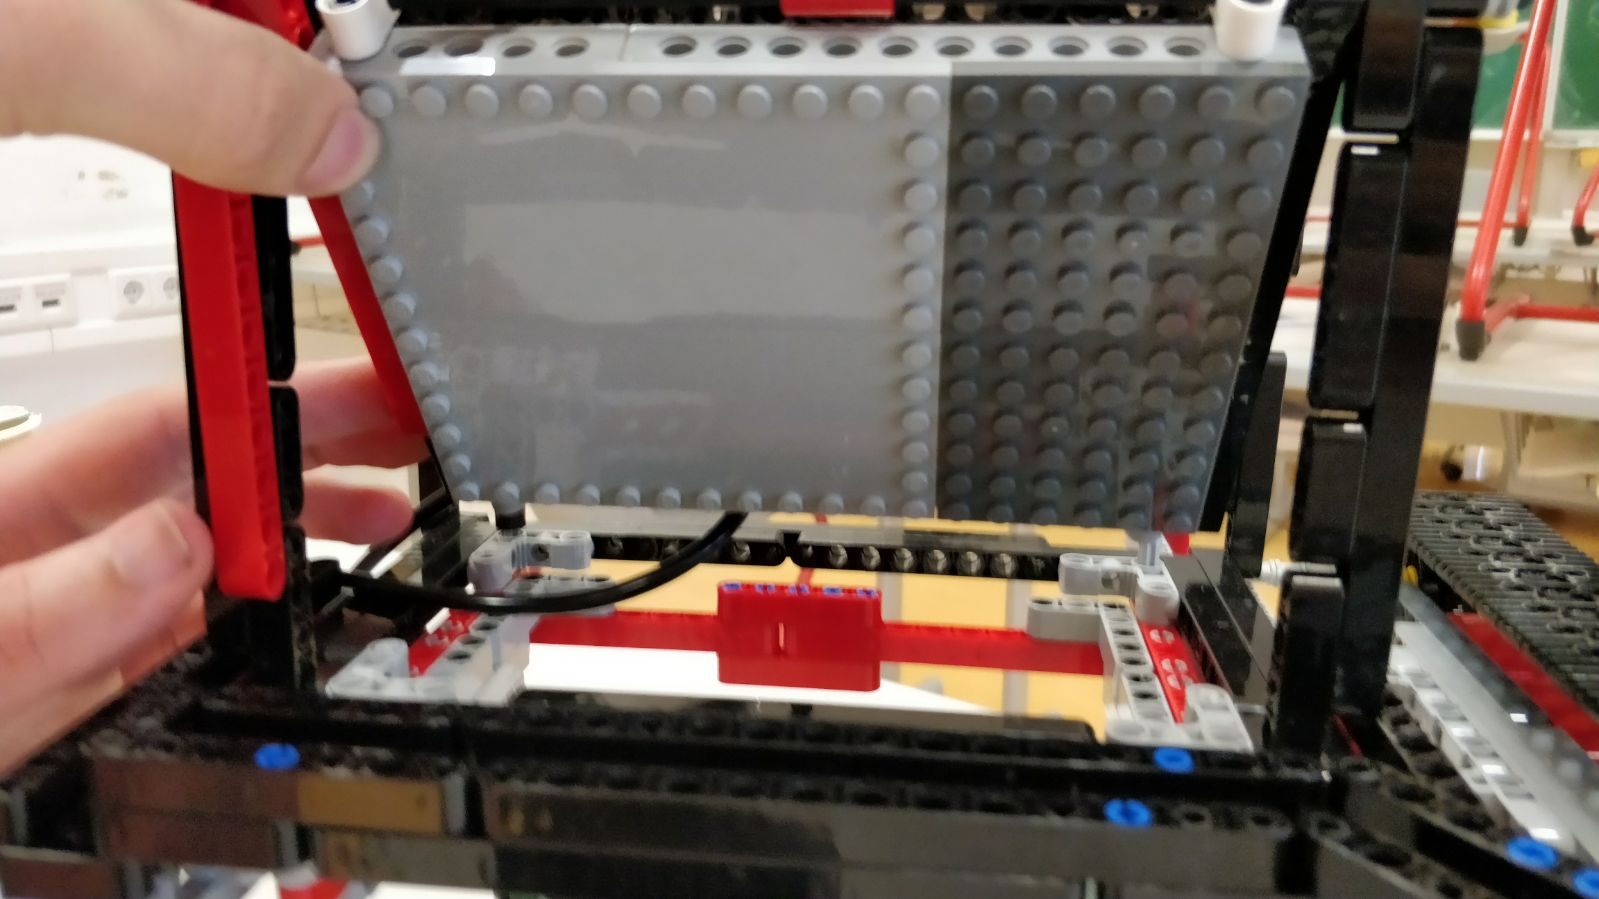
\includegraphics[width=13cm]{Bilder/Ablauf_1_png/Auswurf_5}
\caption{Fertiger Auswurf}
\label{Fertiger Auswurf}
\end{center}
\end{figure}

\subsubsection{Füttern}

\begin{wrapfigure}{r}{0.5\textwidth}
\vspace{-40pt}
  \begin{center}
    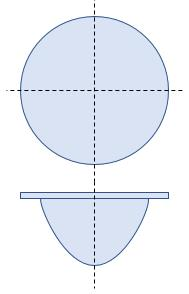
\includegraphics[width=0.17\textwidth]{Bilder/Powerpoint/Loch_Futterschuessel}
  \end{center}
  \caption{Loch Futterschüssel}
  \label{Loch_Futterschuessel}
  \vspace{-10pt}
\end{wrapfigure}

Die Maschine besitzt 5 Futterschüsseln die auf einer drehbaren Platte stehen. Vor dem Füttern wird eine saubere Platte unter der Stelle, wo später die Packung aufgeschnitten wird, positioniert. Während es ausgepresst wird, fliegt das Futter in die Futterschüssel. Wenn der Auspressvorgang beendet ist, wird die Futterschüssel an eine Position bewegt, wo die Katze Zugang zum fressen hat. Die Schüsseln lassen sich einfach aus der Halterung nehmen da sie nur in einem Loch in der Platte liegen. Das hat den Vorteil gegenüber anderen Schüsseln die auf der Platte montiert sind, dass die Katze nicht soweit zur Futterschüssel hat d.h. sie muss nur mit dem Kopf zur Plattenoberfläche und nicht Platte + Schlüsselhöhe, somit spart man je nach Schüssel wertvolle Zentimeter. Die Platte ist mit einer Gummischicht überzogen damit die Schüssel, durch der Kopf der Katze, wenn sie frisst, nicht verrutsch. Sie lässt sich aus der Platte entnehmen, indem der Benutzer mit der Hand die Futterschüssel von unten durch das loch drückt und mit der anderen Hand entnimmt. Danach werden die Schüsseln gewaschen, getrocknet und die Schüssel in das Loch fallen gelassen. Siehe Abbildung: \ref{Loch_Futterschuessel}

\newpage

\subsection{Variante 2: Vor aufgeschnittene Packung }

\subsubsection{Förderband und Kettenglieder}

Beim Förderband erkennt man wo sich die Futterpackungen befinden sollen. Es wird über die zwei Kettenräder eine Kette gespannt. Auf diese Kette werden die Futterpackungen gehängt, dass funktioniert aber nur weil die Kettenglieder einen Rechenwinkel auf jeder Seite hat (siehe Abbildung: \ref{Kettenglied}. Auf diesen Winkel wird eine Aluplatte geschraubt und mit einer anderen Platte festgeklemmt. Die Kette wird mithilfe eines Motors in Bewegung gebracht, damit bewegt sich die Packung immer näher Richtung Walze. Siehe Abbildung: \ref{Foerderband}

\begin{figure}[H]
   \begin{minipage}[hbt]{.3\linewidth} % [b] => Ausrichtung an \caption
      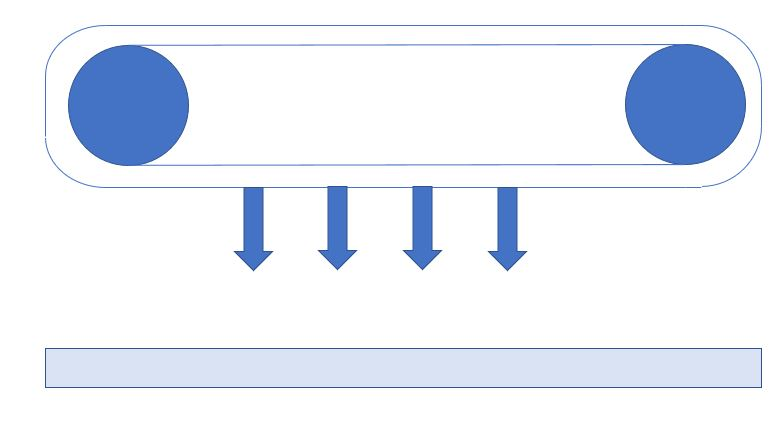
\includegraphics[width=\linewidth]{Bilder/Powerpoint/Foerderband}
      \caption{Foerderband}
      \label{Foerderband}
   \end{minipage}
   \hspace{.3\linewidth}% Abstand zwischen Bilder
   \begin{minipage}[hbt]{.2\linewidth} % [b] => Ausrichtung an \caption
      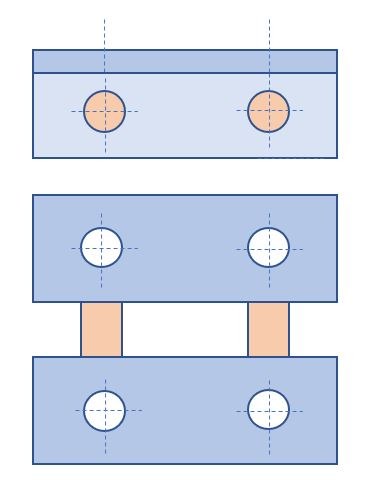
\includegraphics[width=\linewidth]{Bilder/Powerpoint/Kettenglied}
      \caption{Kettenglied}
	  \label{Kettenglied}      
      \end{minipage}
\end{figure}

\subsubsection{Walze}

Nach dem die Futterpackung in Bewegung ist, wird bei einer gewissen Position die Klemme entfernt und durch die Walze gepresst. Die Walze ist innen hohl und wird auf der Welle platziert. Die eine auf der Antriebsseite und die andere auf einer eigen gefertigten Welle. Beide Walzen werden durch eine Feder aneinander gepresst, nur so stark, damit die Halterung, an der die Packung festgemacht ist, durchkommt. Dennoch so stark damit sich die Packung entleert. Die Walze an der eigen gefertigten Welle wird mit zwei Aluplatten und einem Scharnier in Stellung gehalten. Siehe Abbildungen: \ref{Walze}, \ref{Scharnier}.

\begin{figure}[H]
   \begin{minipage}[hbt]{.4\linewidth} % [b] => Ausrichtung an \caption
      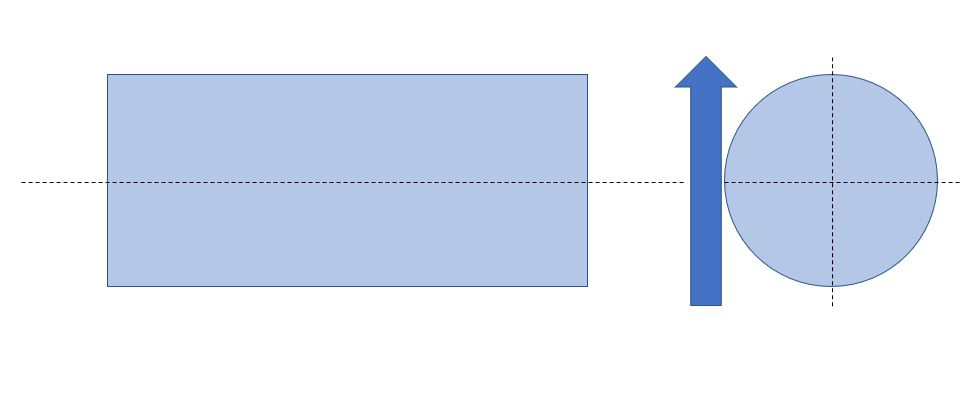
\includegraphics[width=\linewidth]{Bilder/Powerpoint/Walze}
      \caption{Walze}
      \label{Walze}
   \end{minipage}
   \hspace{.2\linewidth}% Abstand zwischen Bilder
   \begin{minipage}[hbt]{.4\linewidth} % [b] => Ausrichtung an \caption
      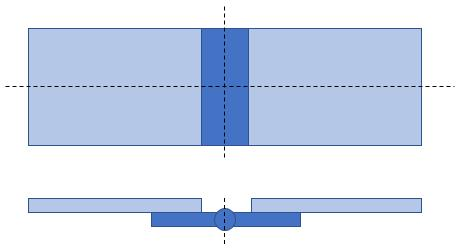
\includegraphics[width=\linewidth]{Bilder/Powerpoint/Schanier}
      \caption{Scharnier}
	  \label{Scharnier}      
      \end{minipage}
\end{figure}

\newpage
\subsubsection{Futterplatte}

\begin{wrapfigure}{r}{0.5\textwidth}
\vspace{-30pt}
  \begin{center}
    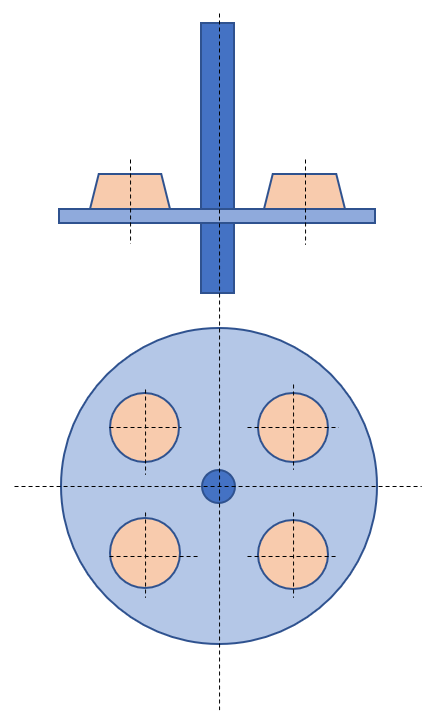
\includegraphics[width=0.32\textwidth]{Bilder/Powerpoint/Futterplatte}
  \end{center}
  \caption{Futterplatte}
  \label{Futterplatte}
  \vspace{-20pt}
\end{wrapfigure}


Nach dem Pressen wird das Futter in die Schüssel gequetscht bzw. es rinnt in die Schüssel. Die Platte hat eine gewisse Anzahl an Schüsseln, je nach Bedarf maximal fünf Schüsseln. Diese sind auf einer Platte platziert, durch den Plattenmittelpunkt geht eine Welle die die Platte nach links und rechts drehen kann. Siehe Abbildung: \ref{Futterplatte}



\subsection{Variante 3: Gefrorenes Futter}

In dieser Variante wurde überlegt, ob man das Futter nicht einfrieren kann, dieses danach aus der Gefriertruhe holt und erwärmt. Der Vorteil hierbei ist es können keine Schädlinge in das Futter gelange da es tiefgefroren ist und es kann die Portionsgröße eingestellt werden wie viel die Katze bekommt da der Benutzer die Menge an Futter selbst bestimmen kann.  Weiters müsste man nicht über das Schneide Problem nachdenken, da es eine knifflige Angelegenheit ist die Packung bei jeden Schnitt perfekt zu schneiden. Der große Nachteil ist der Platzbedarf und der hohe Energieverbrauch der Kühltruhe. Auch die Entnahme des Futters aus der Kühltruhe ist kein leichtes Unterfangen, da man entweder viel mit Magnetzylinder arbeiten muss zur Verschiebung der Abdeckung oder ein Loch aus dem der Greifer das Futter entnimmt und dicht Halten muss, damit die Kühltruhe nicht zu warm wird, alles zerschmiltz und schlussendlich das Futter verdirbt. Hinzuzufügen ist auch noch das Katzen wenn es um Futter geht sehr wählerisch sind und somit wenn das Futter gefroren ist, hat man zu einem  Teil das Kontenzwasser des aufgetauten Futters und zum Anderen schmeckt eingefrorenes Essen anders, also nicht so wie es die Katze gewohnt ist.

\newpage
\section{Aufbauten und Tests}

In diesem Abschnitt der Diplomarbeit werden verschiedene Tests der obigen Varianten zu sehen sein. \\

\subsection{Fütterungsexperiment} 

In diesem Experiment wurde getestet wie lange es Dauert bis eine Packung nur mit Hilfe der Schwerkraft ausläuft. Der Beutel wurde nicht extra erwärmt und wird nur an den beiden unteren Ecken gehalten. Siehe Abbildungen: \ref{Halterung}, \ref{Fütterungs Anfang}, \ref{Fütterungs Mitte}

\begin{figure}[H]
   \begin{minipage}[hbt]{.4\linewidth} % [b] => Ausrichtung an \caption
      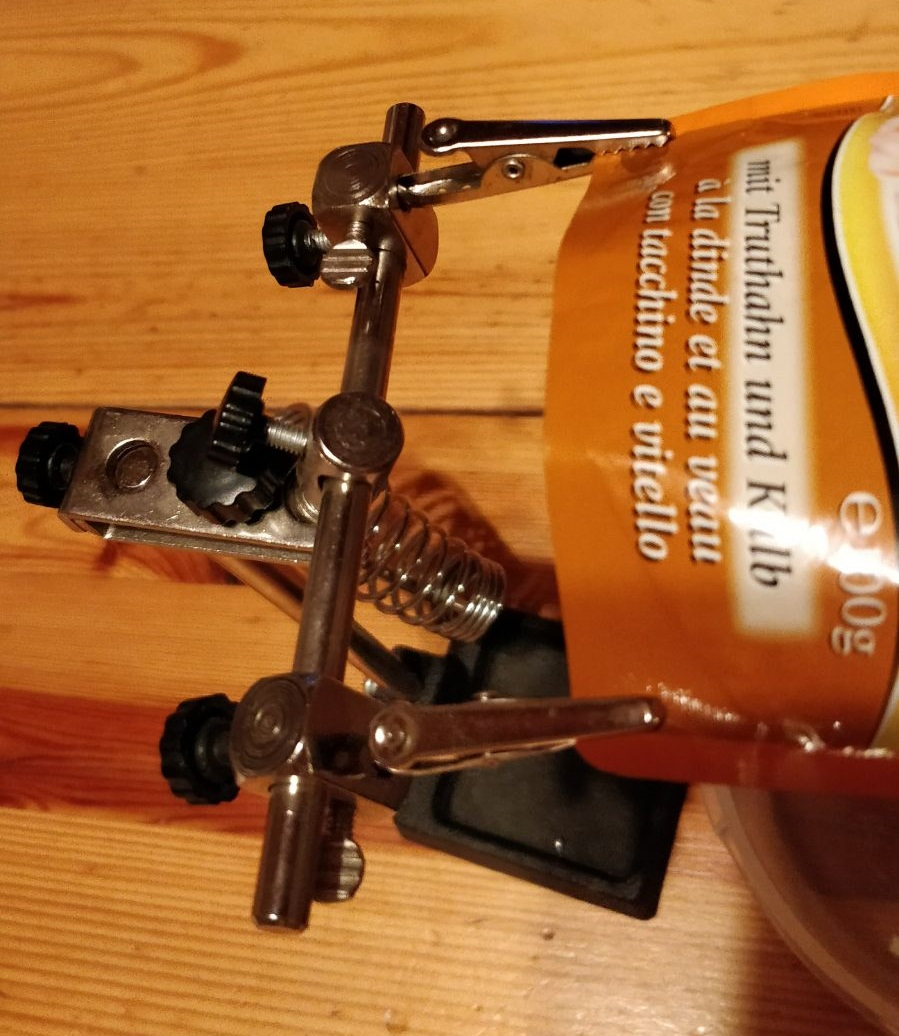
\includegraphics[width=\linewidth]{Bilder/Fuetterungsexperiment/Aufhaengung}
      \caption{Halterung}
      \label{Halterung}
   \end{minipage}
   \hspace{.2\linewidth}% Abstand zwischen Bilder
   \begin{minipage}[hbt]{.4\linewidth} % [b] => Ausrichtung an \caption
      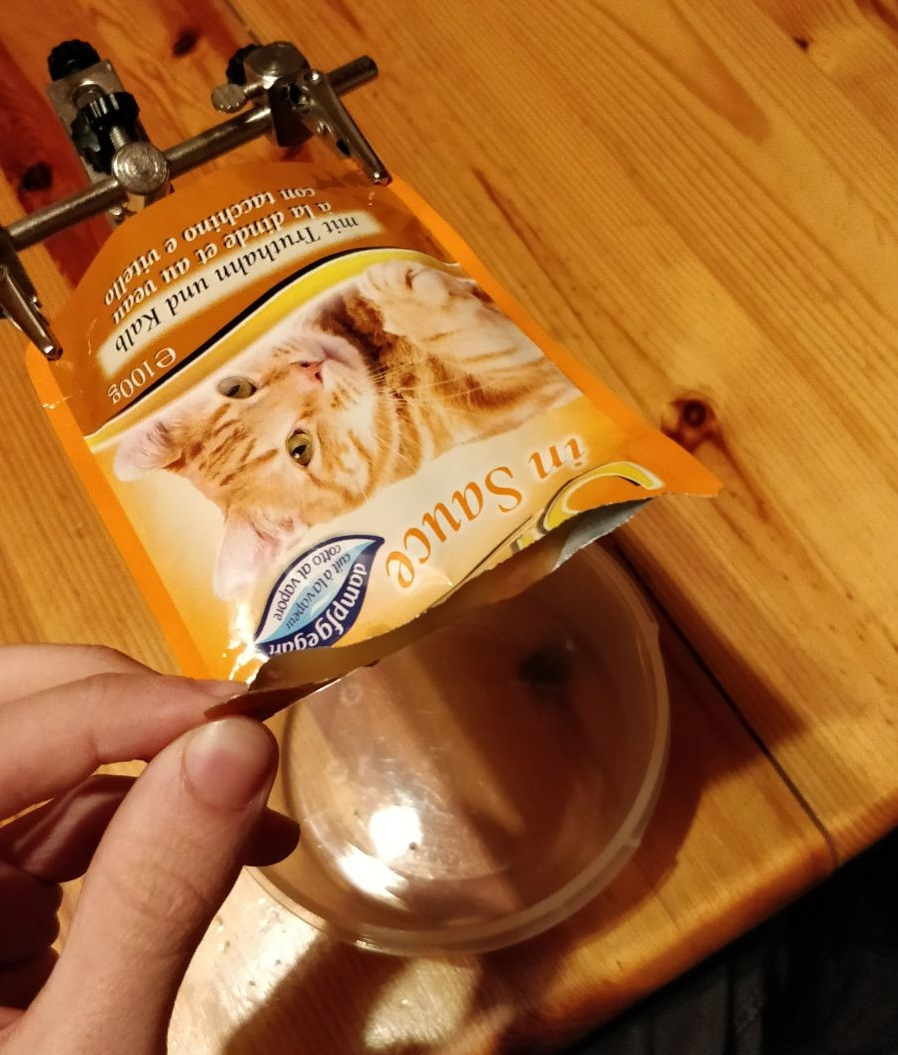
\includegraphics[width=\linewidth]{Bilder/Fuetterungsexperiment/Fuetterungs_Anfang}
      \caption{Fütterungs Anfang}
	  \label{Fütterungs Anfang}      
      \end{minipage}
\end{figure}


\begin{figure}[H]
   \begin{minipage}[hbt]{.3\linewidth} % [b] => Ausrichtung an \caption
      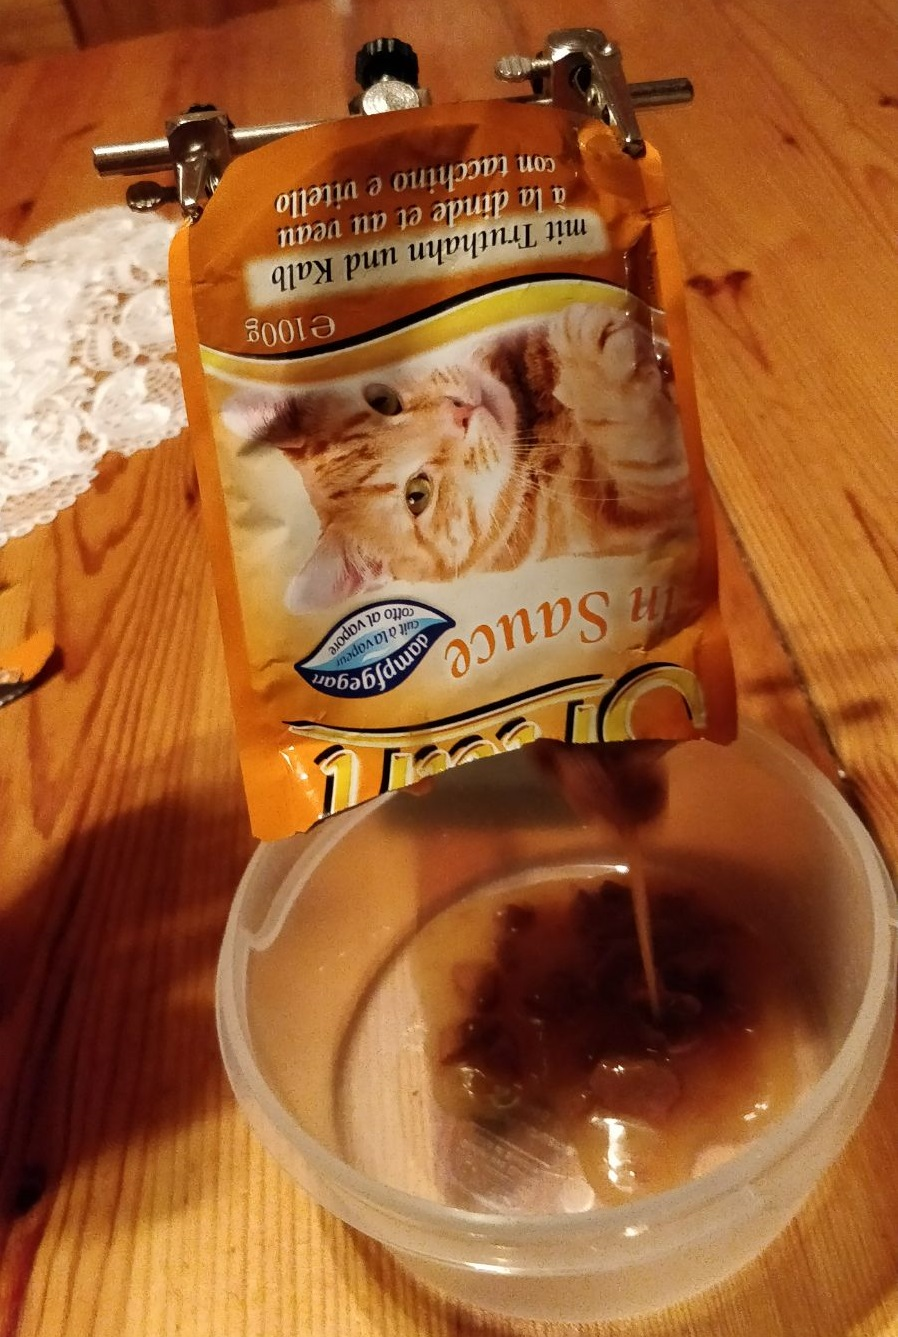
\includegraphics[width=\linewidth]{Bilder/Fuetterungsexperiment/Fuetterungs_Mitte}
      \caption{Fütterungs Mitte}
      \label{Fütterungs Mitte}
   \end{minipage}
   \hspace{.4\linewidth}% Abstand zwischen Bilder
   \begin{minipage}[hbt]{.3\linewidth} % [b] => Ausrichtung an \caption
     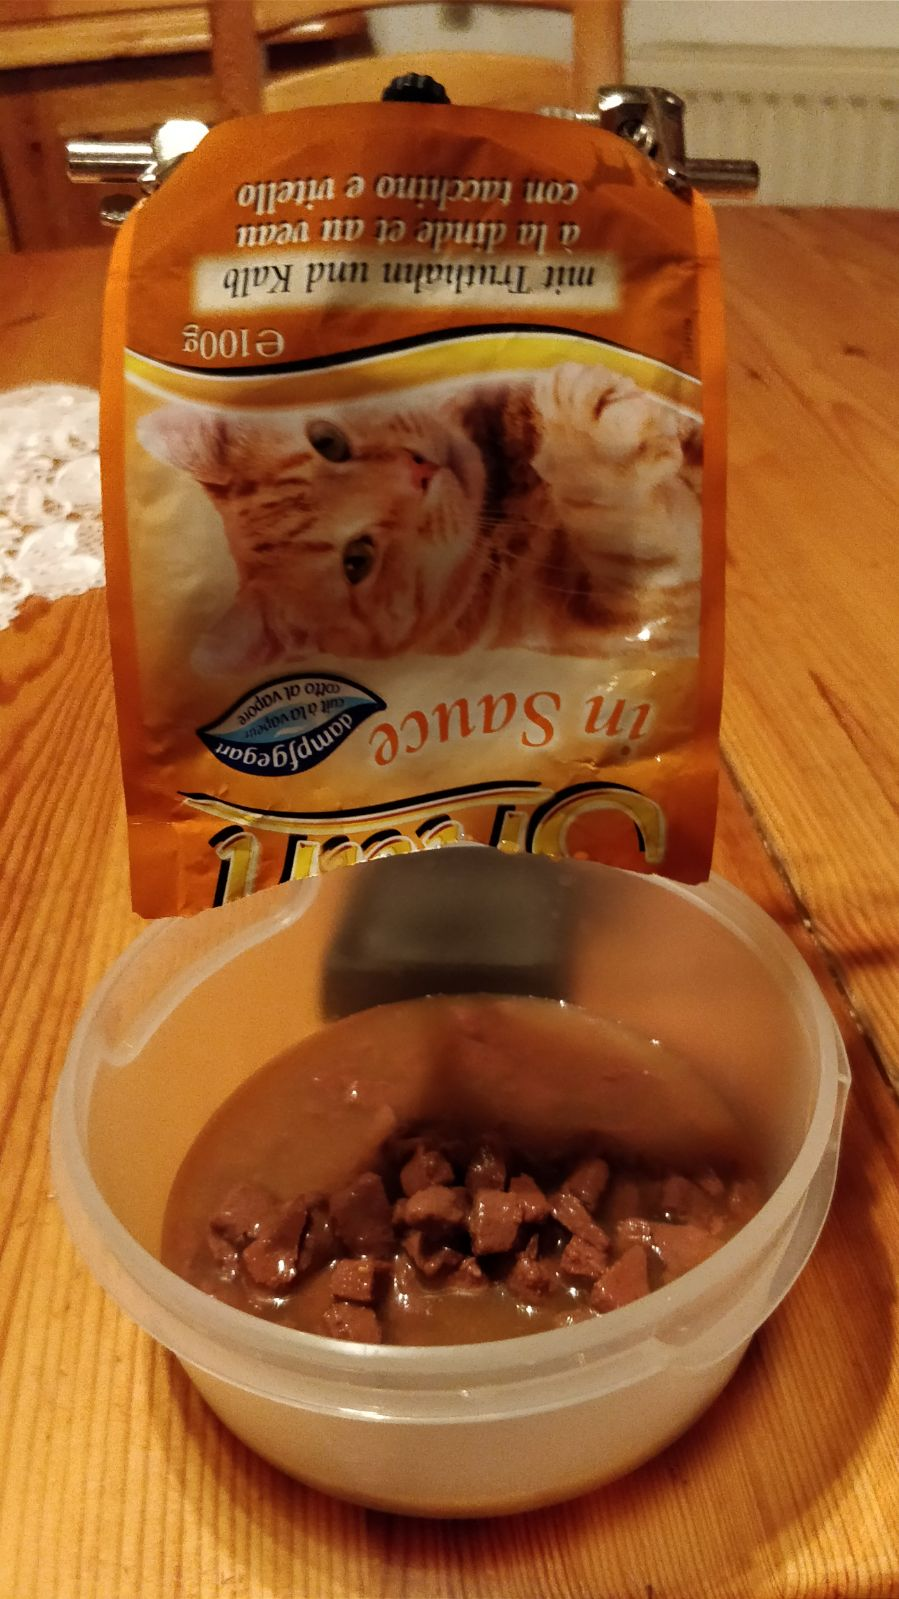
\includegraphics[width=\linewidth]{Bilder/Fuetterungsexperiment/Fuetterungs_Ende}  
      \caption{Fütterungs Ende}
     \label{Fütterungs_Ende}
   \end{minipage}
\end{figure}

In der Abbildung: \ref{Fütterungs_Ende} sieht man das nach 10 Minuten der Inhalte ganz in der Futterschüssel ist, dennoch Tropft es nach.
\newpage
\subsection{Schneideversuch 1.Art der 1.Variante}

Schnitt anhand einer praxischen Anwendung dargestellt. Der Beutel wird mithilfe einer Papierschneidemaschine geschnitten. Siehe Abbildungen: \ref{Einlegen}, \ref{Anfangsschnitt}, \ref{Endschnitt}

\begin{figure}[H]
   \begin{minipage}[hbt]{.3\linewidth} % [b] => Ausrichtung an \caption
      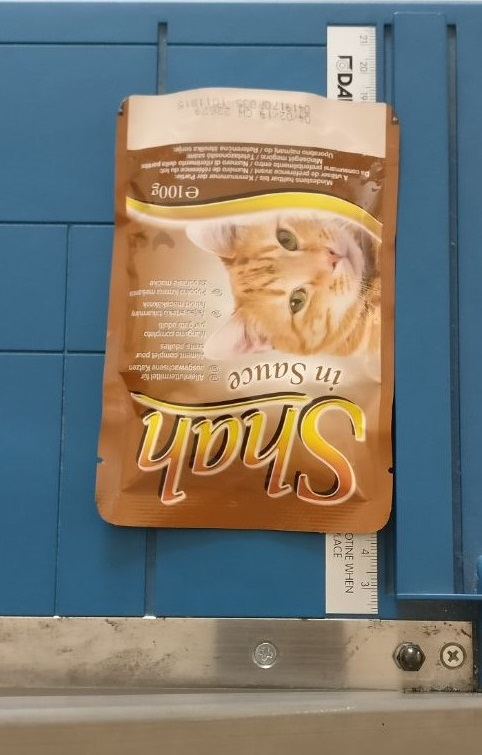
\includegraphics[width=\linewidth]{Bilder/Schneideversuch_1.Art/Einlegen}
      \caption{Einlegen}
      \label{Einlegen} 
   \end{minipage}
   \hspace{.2\linewidth}% Abstand zwischen Bilder
   \begin{minipage}[hbt]{.5\linewidth} % [b] => Ausrichtung an \caption
      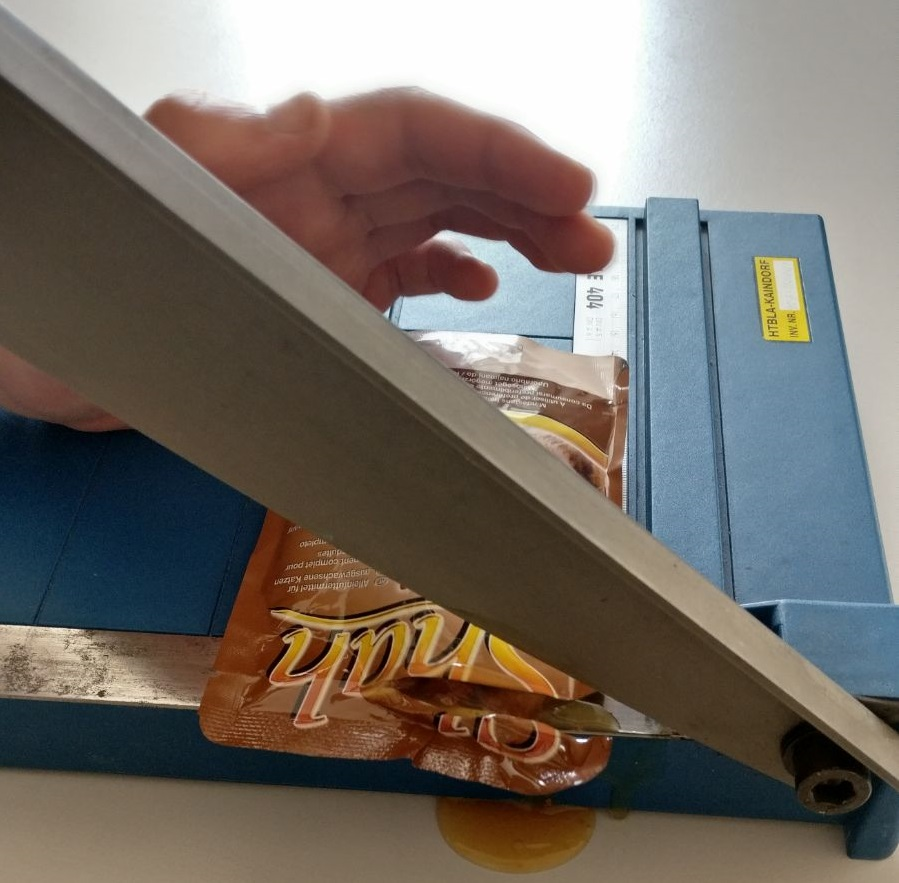
\includegraphics[width=\linewidth]{Bilder/Schneideversuch_1.Art/Anfangsschnitt}
      \caption{Anfangsschnitt}
      \label{Anfangsschnitt} 
   \end{minipage}
\end{figure}

\begin{figure}[H]
\begin{center}
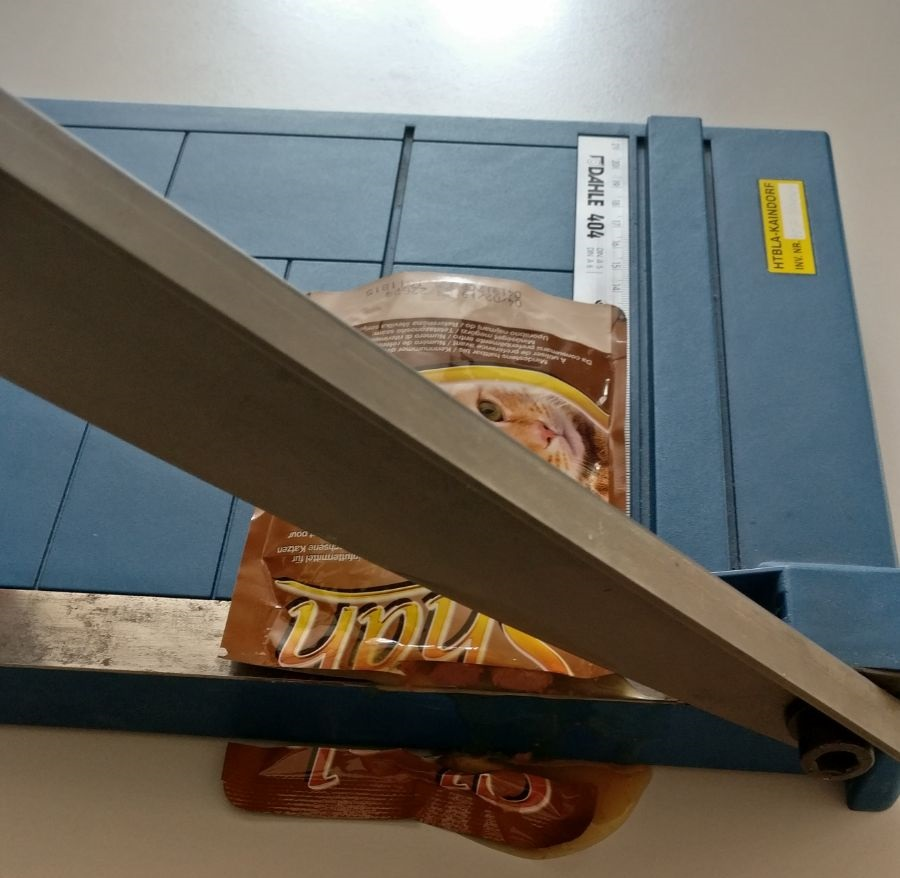
\includegraphics[width=7cm]{Bilder/Schneideversuch_1.Art/Endschnitt}
\caption{Endschnitt}
\label{Endschnitt} 
\end{center}
\end{figure}
\newpage
\subsection{Schneideversuch 2.Art der 1.Variante}

Mit einem Metallwerkzeug mit Wellenschliffartiger Kante wird der Futterbeutel entlang der Oberseite aufgeschnitten. Um die Packung vollständig geöffnet zu haben, mussten mehrere Schnitte verwendet werden. Siehe Abbildung: \ref{Schneidemittel}

\begin{figure}[H]
   \begin{minipage}[hbt]{.3\linewidth} % [b] => Ausrichtung an \caption
      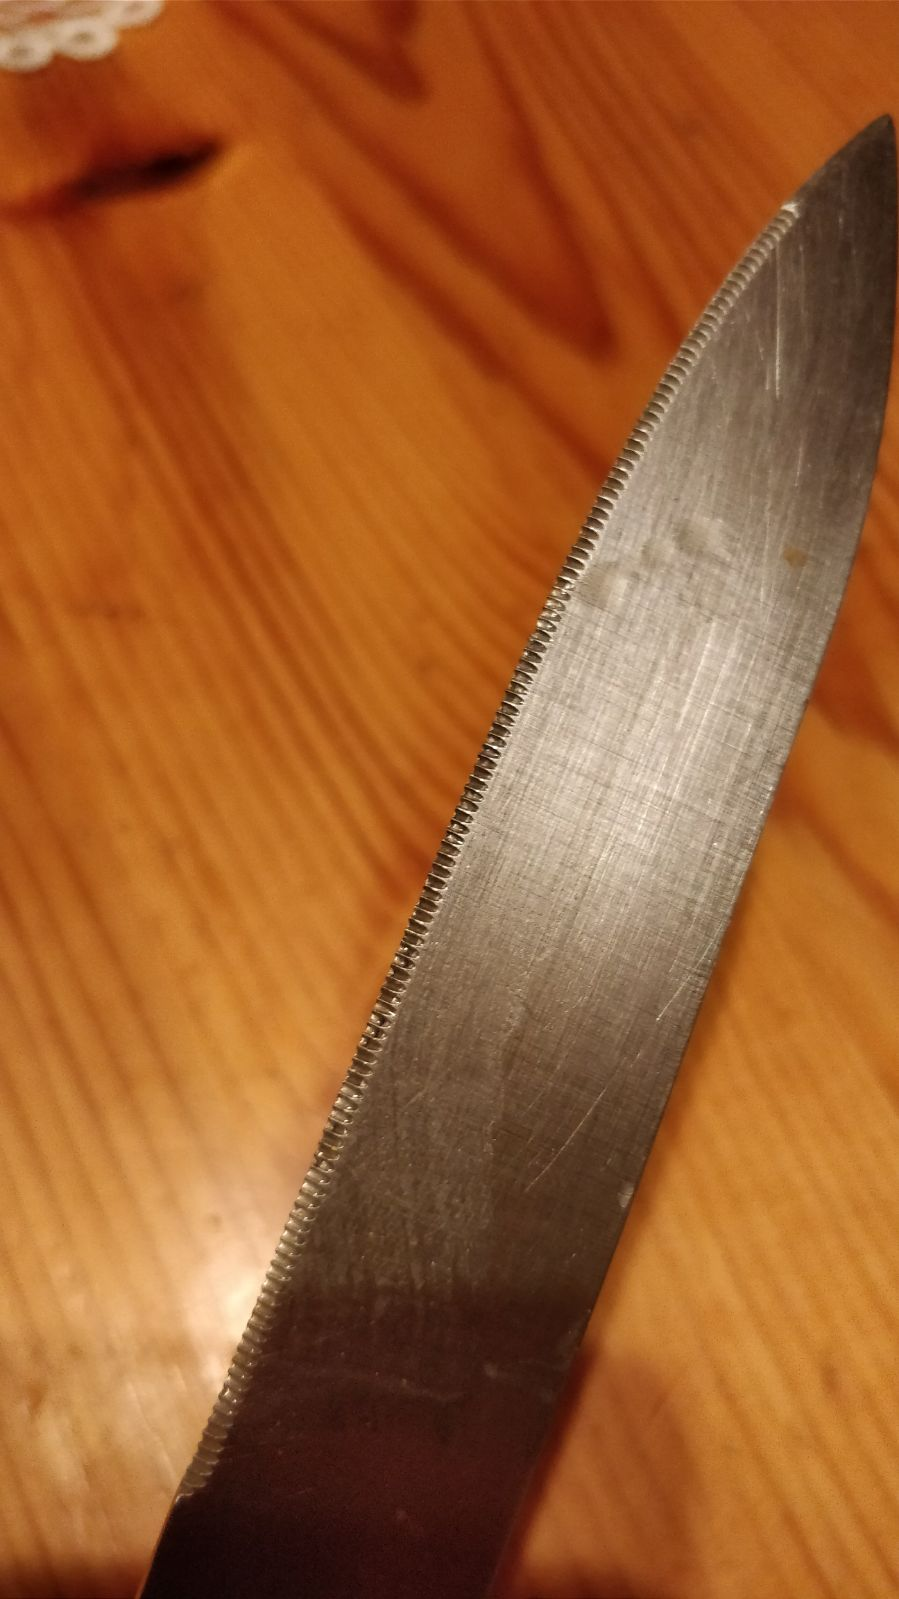
\includegraphics[width=\linewidth]{Bilder/Schneideversuch_2.Art/Schneidemittel}
      \caption{Schneidemittel}
      \label{Schneidemittel} 
   \end{minipage}
   \hspace{.4\linewidth}% Abstand zwischen Bilder
   \begin{minipage}[hbt]{.3\linewidth} % [b] => Ausrichtung an \caption
      
\includegraphics[width=\linewidth]{Bilder/Schneideversuch_2.Art/Anfangsschnitt}
      \caption{Anfangsschnitt 2.Art}
      \label{Nach 3 Schnitten}
   \end{minipage}
\end{figure}

In der Abbildung: \ref{Nach 3 Schnitten} erkennt man wie offen die Packung nach 3 Schnitten ist.

\begin{figure}[H]
   \begin{minipage}[hbt]{.4\linewidth} % [b] => Ausrichtung an \caption
      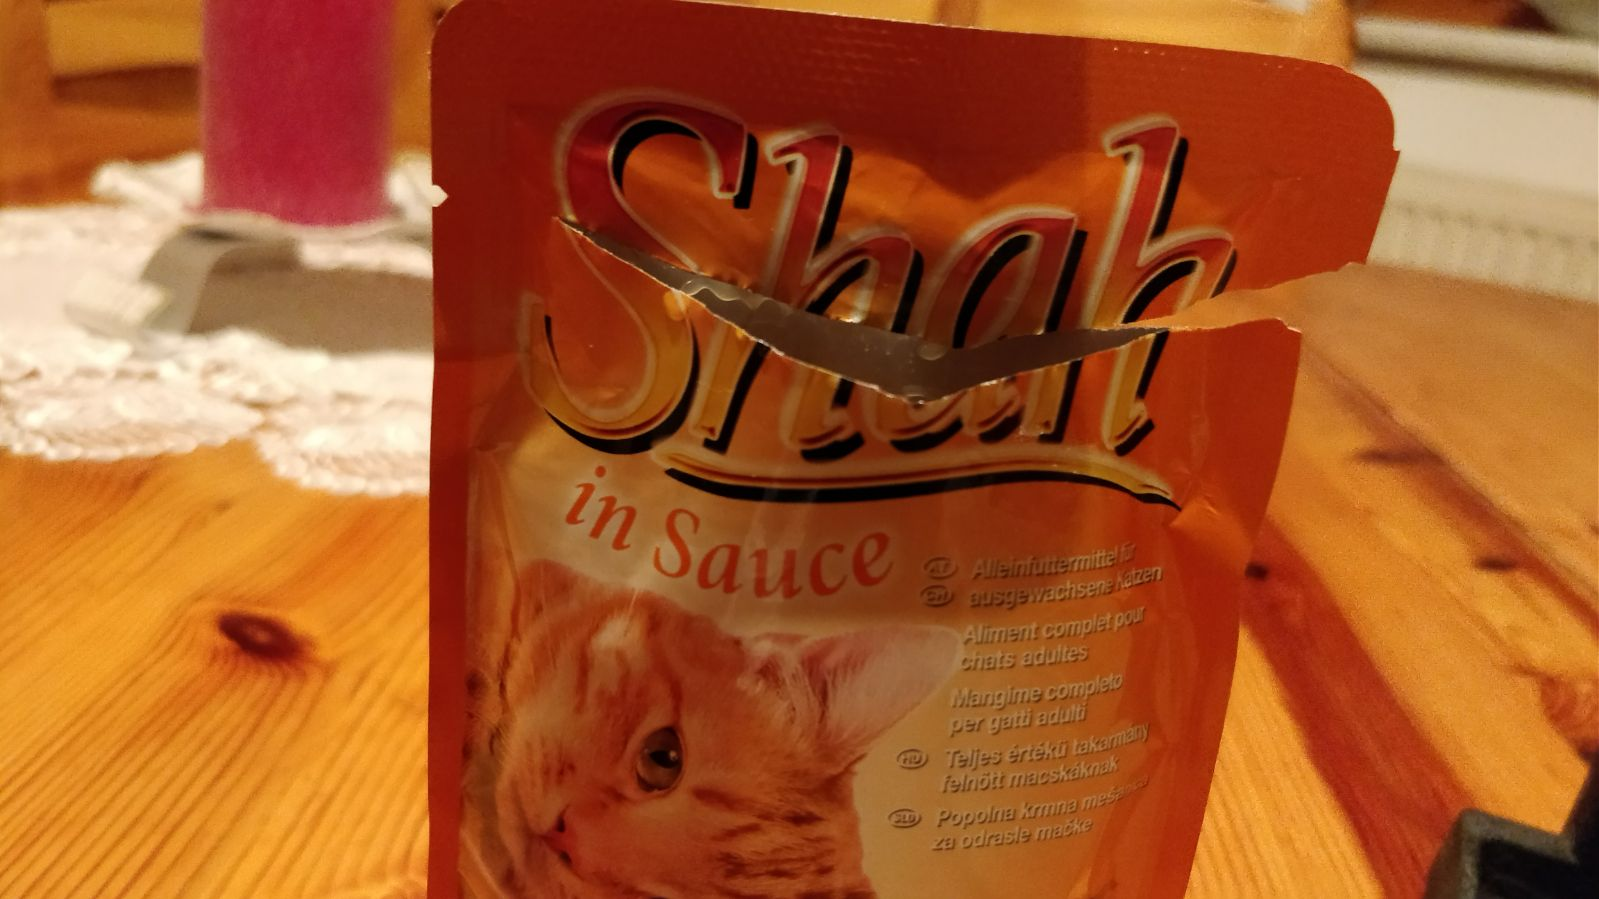
\includegraphics[width=\linewidth]{Bilder/Schneideversuch_2.Art/Mittelschnitt}
      \caption{Mittelschnitt 2.Art}
      \label{Nach 6 Schnitten}
   \end{minipage}
   \hspace{.2\linewidth}% Abstand zwischen Bilder
   \begin{minipage}[hbt]{.4\linewidth} % [b] => Ausrichtung an \caption
      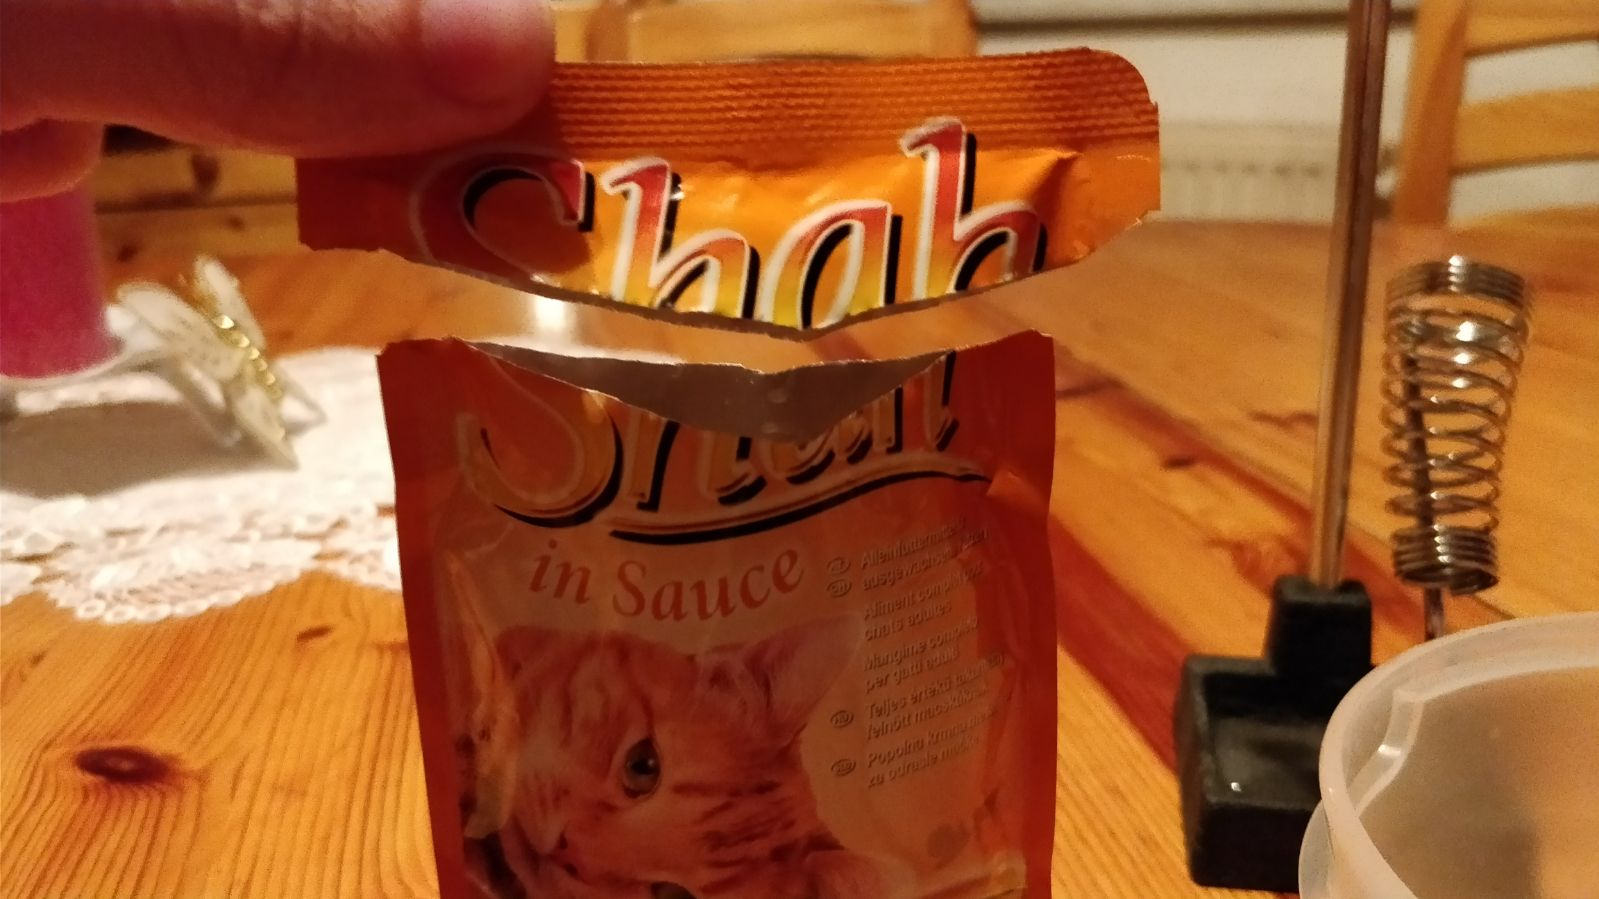
\includegraphics[width=\linewidth]{Bilder/Schneideversuch_2.Art/Endschnitt}
      \caption{Endschnitt 2.Art}
      \label{Nach 9 Schnitten}
   \end{minipage}
\end{figure}
In der Abbildung: \ref{Nach 6 Schnitten} erkennt man wie offen die Packung nach 6 Schnitten ist.\\

In der Abbildung: \ref{Nach 9 Schnitten} wurde die Packung nach 9 Schnitten vollständig geöffnet.
\subsection{Dichtheitsexperiment der Hebelklemme}

\section{Vergleich der Varianten}
\subsection{Klemmen}
\subsubsection{Einfache Klemme}

\begin{wrapfigure}{r}{0.5\textwidth}
\vspace{-20pt}
  \begin{center}
    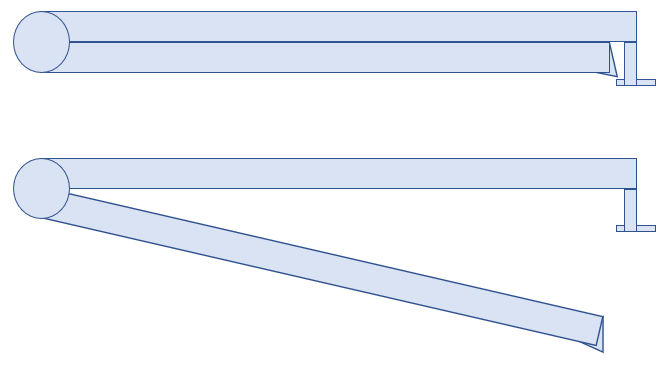
\includegraphics[width=0.32\textwidth]{Bilder/Powerpoint/Einfach_Klemme}
  \end{center}
  \caption{Einfache Klemme}
  \label{Einfache Klemme}
  \vspace{-10pt}
\end{wrapfigure}

Die einfach Klemme ist für gewöhnliche Verpackungen gut zu nutzen jedoch ist sie für unsere Variante nicht zu gebrauchen, dadurch Kunstoff nicht so stabil wie Metall ist drück sie die Packung an manchen Stellen zu wenig zusammen und an diesen Stellen kann Flüssigkeit austreten. Außerdem hält sie bei Zugbelastung nur wenig stand. Siehe Abbildung: \ref{Einfache Klemme}

\subsubsection{Hebel Klemme} 

\begin{wrapfigure}{r}{0.5\textwidth}
\vspace{-30pt}
  \begin{center}
    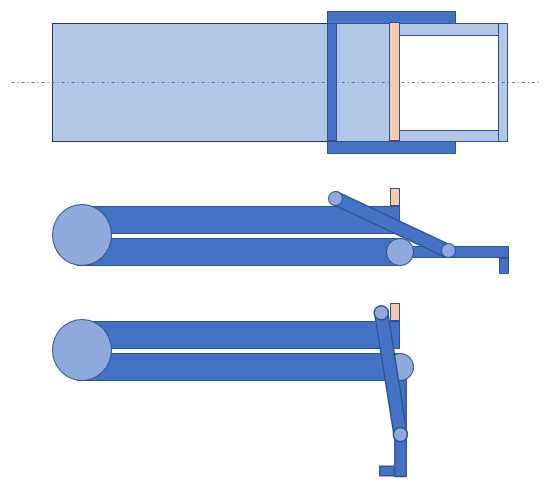
\includegraphics[width=0.32\textwidth]{Bilder/Powerpoint/Hebel_Klemme}
  \end{center}
  \caption{Hebel Klemme}
  \label{Hebel Klemme}
  \vspace{-10pt}
\end{wrapfigure}

Die Hebel Klemme ist für diese Diplomarbeit die bevorzugte Methode sie kann viel Druck auf die Packung ausüben sodass keine Flüssigkeit entrinnen kann. Außerdem lässt sich durch den Hebel mit wenig Kraft die Klemme öffnen. Weiters können die Klemmen auf einer Stange aufgesammelt werden und liegen nicht an unerwünschten Positionen an denen man nicht herankommt. Siehe Abbildung:    
 \ref{Hebel Klemme}
 \vspace{40pt}


\subsubsection{Gummiband Klemme}
 
\begin{wrapfigure}{r}{0.5\textwidth}
\vspace{-40pt}
  \begin{center}
    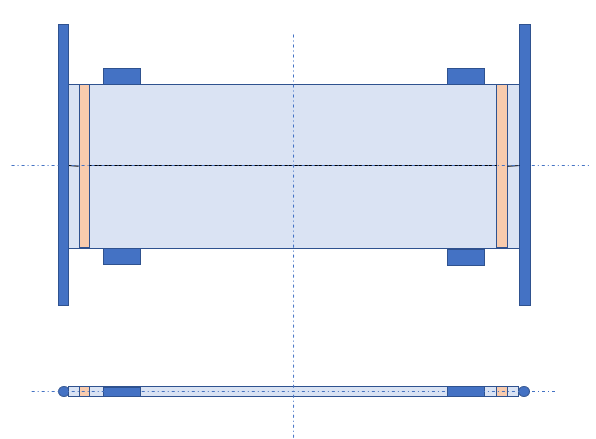
\includegraphics[width=0.30\textwidth]{Bilder/Powerpoint/Gummiband_Klemme}
  \end{center}
  \caption{Gummiband Klemme}
  \label{Gummiband Klemme}
  \vspace{-20pt}
\end{wrapfigure}

Die Gummiband Klemme hat eine starke Klemmkraft, dies Schützt vor dem Aufplatzen der Verpackung. Das Problem dieser Variante ist das das Gummiband spröder werden kann und irgendwann reißen, also ein hoher Verschleiß. Die Klemmen kann man auch nicht kontrolliert sammeln und somit sind sie schwerer zugänglich.

\subsection{Futterschüsseln}

\subsubsection{Drehfutterplatte}

\begin{wrapfigure}{r}{0.5\textwidth}
\vspace{-40pt}
  \begin{center}
    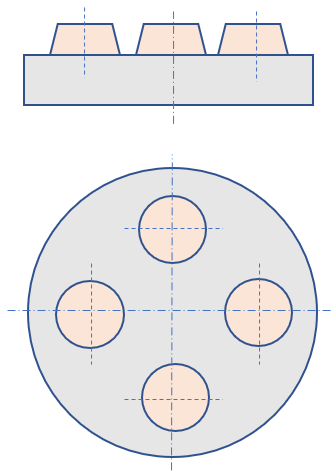
\includegraphics[width=0.25\textwidth]{Bilder/Powerpoint/Drehplatte}
  \end{center}
  \caption{Drehplatte}
  \label{Drehplatte}
  \vspace{-20pt}
\end{wrapfigure}

Die Drehplatte besteht aus fünf Schüsseln man kann pro Schüssel die Katze 2-mal am Tag füttern abends und morgens. Dadurch hat die Katze jeden Tag einen neue Schüssel und falls sie nicht frisst muss sie nicht Hunger leiden. Auf einer Welle wird eine Platte befestigt 
darin werden fünf Löcher geschnitten und die Schüssel hinein gelegt. Die Drehplatte wird mit einen Schneckengewinde in die gewünschten Position gebracht. Siehe Abbildung:  	
 \ref{Drehplatte} \vspace{+80pt}
 

\subsubsection{Futterplatte Zylinder}

\begin{wrapfigure}{r}{0.5\textwidth}
\vspace{-50pt}
  \begin{center}
    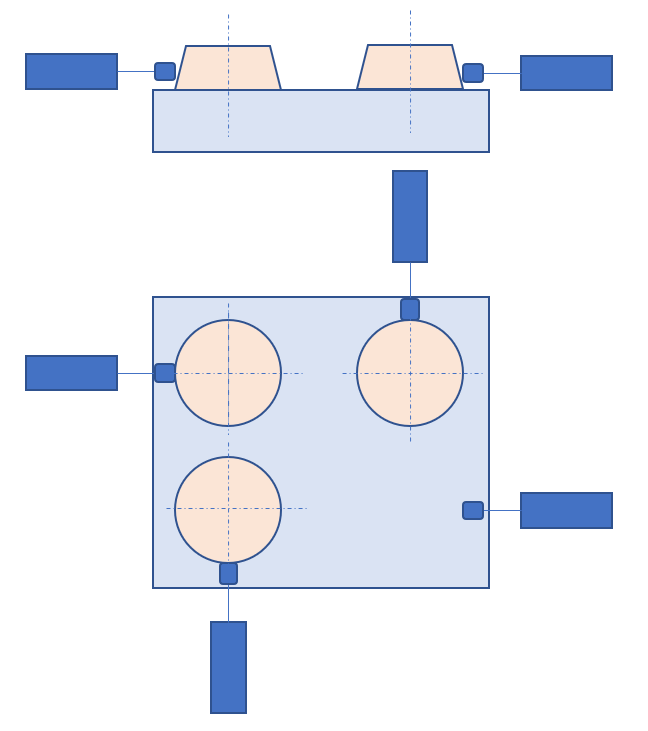
\includegraphics[width=0.32\textwidth]{Bilder/Powerpoint/Platte_Zylinder}
  \end{center}
  \caption{Platte Zylinder}
  \label{Platte Zylinder}
  \vspace{-20pt}
\end{wrapfigure}

Die Futterplatte mit Zylinder ist die umständlichste Variante. Es ist eine viereckige Platte auf der Schienen für das schieben der Futterschüsseln platziert sind. Diese werden von Magnetzylindern angeschoben. Der Nachteil hierbei ist, man benötigt viele Bauteile und alle Zylinder müssen zugleich arbeiten um die Futterschüssel zur richtigen Position zu führen. Siehe Abbildung: \ref{Platte Zylinder} 


\newpage
\subsubsection{Platte mit einer Schüssel}

\begin{wrapfigure}{r}{0.5\textwidth}
\vspace{-40pt}
  \begin{center}
    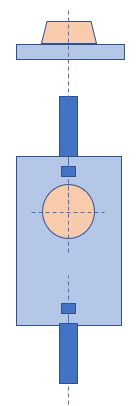
\includegraphics[width=0.17\textwidth]{Bilder/Powerpoint/Einschuessel_platte}
  \end{center}
  \caption{Einschüsselplatte}
  \label{Schüssel Eins}
  \vspace{-10pt}
\end{wrapfigure}

Die Platte mit nur einer Schüssel ist leicht zu realisieren da sie nur wenige Bauteile benötigt. Das wäre zum Einem die Platte auf der die Futterschüssel mit einer Schiene darauf platziert ist. Sowohl als auch die zwei Magnetzylinder die die Futterschüssel in die Anfangs und Endposition bringt. Jedoch ein großer Nachteil weswegen diese Methode nicht in Frage kommt ist, wenn die Katze nach dem Füttern nicht frisst dann bleibt der Inhalt in der Schale und trocknet ein oder es kommt Ungeziefer hinein. Das hat zu Folge das die Schüssel jeden Tag befüllt wird und übergeht. Siehe Abbildung: \ref{Schüssel Eins} 



\subsection{Futtermagazine}

\subsubsection{Futtermagazin Horizontal}

\begin{wrapfigure}{r}{0.5\textwidth}
\vspace{-40pt}
  \begin{center}
    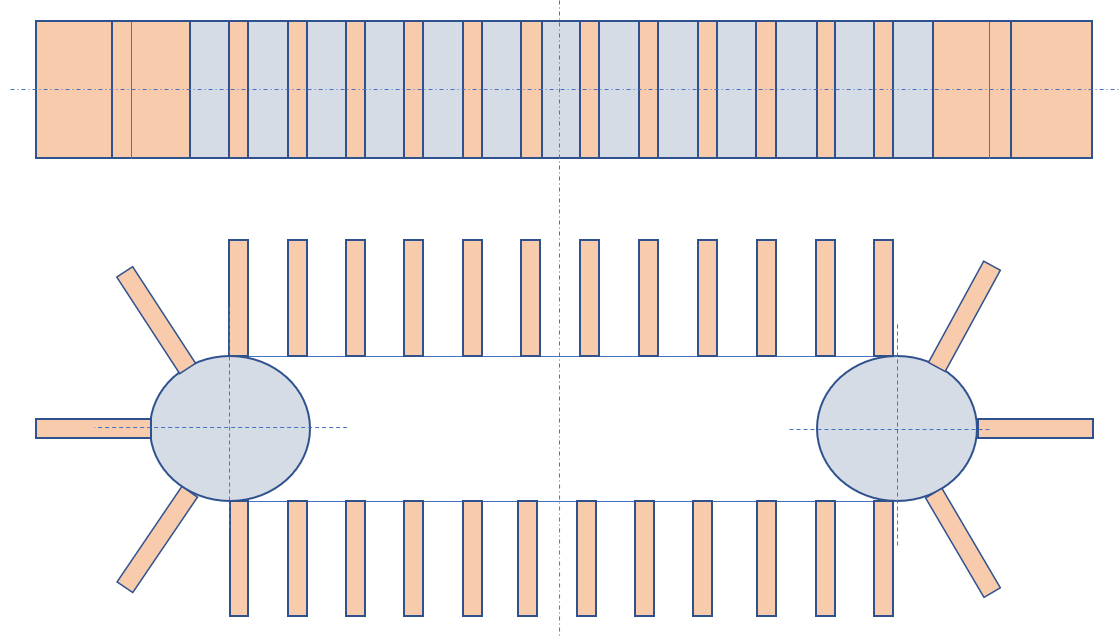
\includegraphics[width=0.30\textwidth]{Bilder/Powerpoint/Futtermagazin_horizontal}
  \end{center}
  \caption{Futtermagazin Horizontal}
  \label{Magazin Horizontal}
  \vspace{-10pt}
\end{wrapfigure} 

Das Futtermagazin Horizontal wäre für die erste Variante optimal. Da man den gewünschten Vorrat an Futterpackungen in die abgetrennten Räume platziert. Somit ist es einfach die gewünschte Position anzufahren und mit einen Greifer in die Schneideposition zu bringen. Der Aufbau ist wie ein Förderband, zwei Räder, ein Band mit oben platzierten Trennwänden und ein Motor der dieses Futtermagazin in Bewegung bringt. Zu beachten wäre wie die Futterpackungen ins Magazin eingelegt werden, nämlich mit der dünneren Fläche mit der Einkerbung die der Hersteller angegeben hat. Siehe Abbildung: \ref{Magazin Horizontal}
\newpage
\subsubsection{Futtermagazin Vertikal}

\begin{wrapfigure}{r}{0.5\textwidth}
\vspace{-40pt}
  \begin{center}
    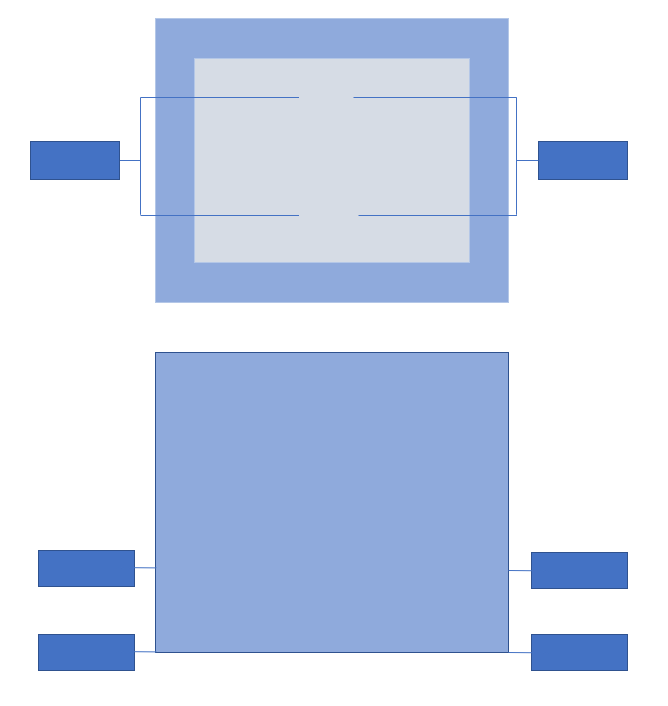
\includegraphics[width=0.26\textwidth]{Bilder/Powerpoint/Futtermagazin_vertikal}
  \end{center}
  \caption{Futtermagazin Vertikal}
  \label{Magazin Vertikal}
  \vspace{-10pt}
\end{wrapfigure}

Das Futtermagazin Vertikal ist ein rechteckiges Gehäuse an denen 4 Magnetzylinder platziert werden. In dieser Box kommen die 10 Futterpackungen. Der Ablauf funktioniert in einer gewissen Reihenfolge. Zuerst öffnet sich der erste linke Magnetzylinder danach der gegenüberliegende zweite Magnetzylinder. Daraufhin gelangt die erste Futterpackung auf die unteren Zylinder. Nach diesem Schritt schließen sich die beiden Magnetzylinder wieder, damit die anderen Packungen nach den öffnen der unteren Magnetzylinder nicht durch die Maschine fallen. Daraufhin wenn der Fütterungsbefehl kommt öffnen sich die unteren Zylinder und die Packung gleitet über ein Blech zur Schnittfläche. Der große Nachteil dieser Methode ist das immer wieder Fehler auftreten können. Die Futterpackung kann falsch an der Schneidfläche ankommen bzw. sich an einem bestimmten Ort verkeilen. Siehe Abbildung: \ref{Magazin Vertikal}

\section{Konstruktion der Wahlvariante und Details}

\subsection{Drehplatte}

\begin{wrapfigure}{r}{0.5\textwidth}
\vspace{-20pt}
  \begin{center}
    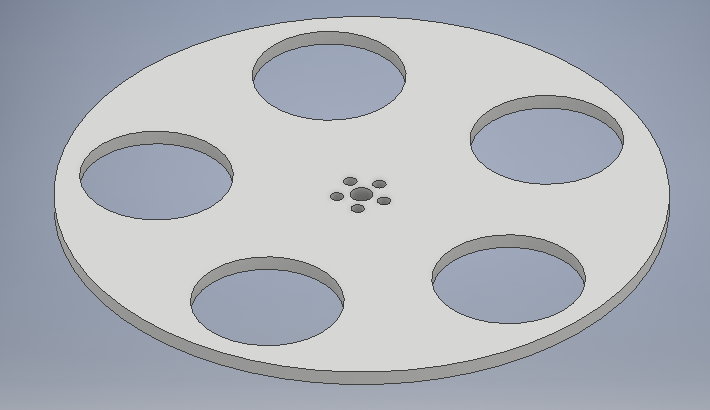
\includegraphics[width=0.30\textwidth]{Bilder/Inventor/Drehplatte}
  \end{center}
  \caption{Drehplatte Inventor}
  \label{Drehplatte_Inventor}
  \vspace{-10pt}
\end{wrapfigure}

Die Drehplatte besteht aus Aluminium und ist 10mm dick. Es werden 5 Löcher für die Schüsseln ausgeschnitten und in der Mitte ist ein Loch, in der eine Stahlwelle durch geht. Die Stahlwelle wurde deshalb ausgewählt, da sie erstens stabiler ist und somit kleiner bzw. mit kleinerem Durchmesser gewählt werden kann. Zweitens ist der Vierkant der in den Motor geht 4x4x20, dies ist für Aluminum sehr schmal da große Kräfte auftreten können und der Stift abreißen kann. Die Drehplatte wird auf der Welle mit einem Flunsch befestigt damit das verutschen nach oben, unten und zur Seite gesichert ist. Siehe Abbildung: \ref{Drehplatte_Inventor}

\begin{wrapfigure}{r}{0.5\textwidth}
\vspace{-20pt}
  \begin{center}
    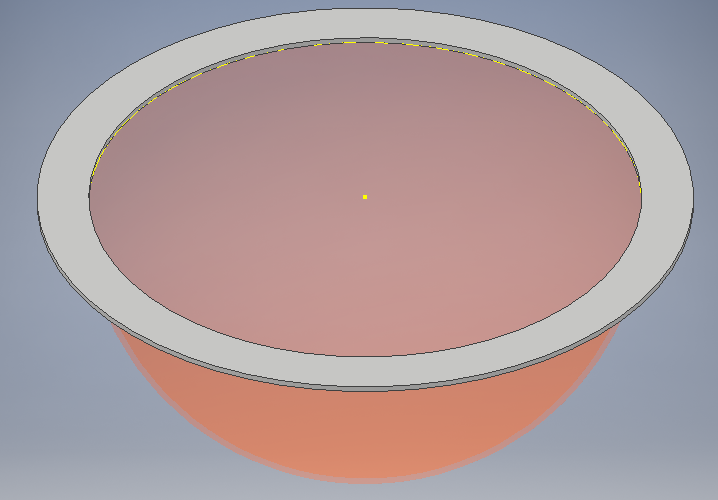
\includegraphics[width=0.26\textwidth]{Bilder/Inventor/Schuessel}
  \end{center}
  \caption{Futterschüssel Inventor}
  \label{Futterschuessel_Inventor}
  \vspace{-10pt}
\end{wrapfigure}

Die Futterschüssel hat deshalb einen Rand damit sie in ein Loch gelegt werden kann ohne dass sie durchfliegt, dennoch lässt sie sich leicht raus nehmen und reinigen. Durch eine rutschfeste Unterlage verrutsch die Schüssel nicht, auch wenn die Katze daraus frisst und sie mit Kraft die Schüssel zu verschieben versucht. Siehe Abbildung: \ref{Futterschuessel_Inventor}.

\subsection{Förderband und Kettenglied}

\begin{wrapfigure}{r}{0.5\textwidth}
\vspace{-20pt}
  \begin{center}
    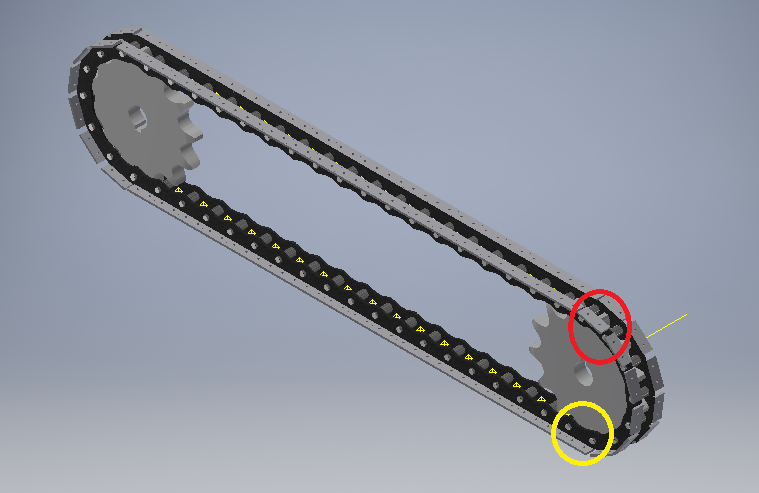
\includegraphics[width=0.26\textwidth]{Bilder/Inventor/Kette}
  \end{center}
  \caption{Kette Inventor}
  \label{Kette_Inventor}
  \vspace{-10pt}
\end{wrapfigure}

Konstruktion der Kette.

\begin{wrapfigure}{r}{0.5\textwidth}
\vspace{-20pt}
  \begin{center}
    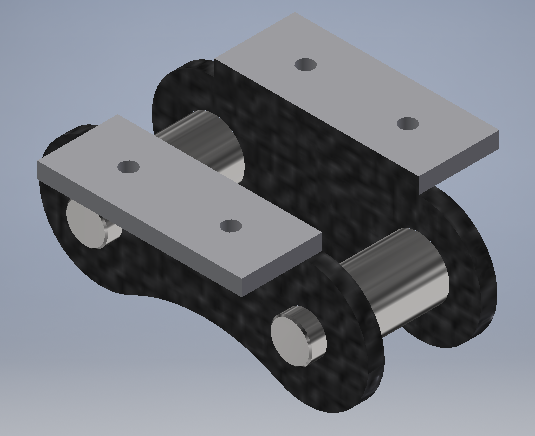
\includegraphics[width=0.26\textwidth]{Bilder/Inventor/Kettenglied}
  \end{center}
  \caption{Kettenglied Inventor}
  \label{Kettenglied_Inventor}
  \vspace{-10pt}
\end{wrapfigure}

Das Kettenglied ist im Handel erhältlich. Die Anfertigung hat auf der Seite einen Rechtenwinkel auf denen Aluplatten platziert sind. Auf diese Aluplatten wird der Futterbeutel platziert.


\subsection{Walze}
\section{Berechnung und Dimensionierung}
\section{Simulation}
\section{Bedienung und Wartung}
\section{Selbstkritische Analyse und Ausblick}

